% Compile from article/: pdflatex main; biber main; pdflatex main; pdflatex main
\documentclass[11pt,a4paper]{article}
\usepackage[utf8]{inputenc}
\usepackage[T1]{fontenc}
\usepackage[english]{babel}
\usepackage[margin=25mm]{geometry}
\usepackage{newtxtext,newtxmath}
\renewcommand{\ttdefault}{lmtt}
\usepackage{amsmath,mathtools}
\usepackage{graphicx,booktabs,ragged2e,etoolbox,placeins,needspace}
\usepackage{tabularray}
\UseTblrLibrary{booktabs,siunitx}
\usepackage[font=small,labelfont=bf,labelsep=period]{caption}
\usepackage{csquotes}
\usepackage[backend=biber,style=authoryear,maxcitenames=2,maxbibnames=99,doi=true,isbn=false,url=false]{biblatex}
\addbibresource{references.bib}
\usepackage{xurl}
\usepackage[hidelinks]{hyperref}
\usepackage{microtype}
\SetTblrInner[booktabs]{width=\textwidth,row{1}={font=\bfseries},hline{1,Z}={0.8pt},hline{2}={0.4pt}}
\SetTblrStyle{remark-text}{font=\footnotesize}
\SetTblrStyle{remark-tag}{font=\footnotesize\itshape}
\newenvironment{tablenotes}[1][Note]{\par\medskip\begingroup\footnotesize\noindent\textit{#1:} }{\par\endgroup}
\newenvironment{figurenotes}[1][Note]{\par\medskip\begingroup\footnotesize\noindent\textit{#1:} }{\par\endgroup}
\newlength{\baselinedist}\setlength{\baselinedist}{\baselineskip}
\setlength{\emergencystretch}{2em}
\setcounter{topnumber}{3}\setcounter{totalnumber}{4}
\renewcommand{\topfraction}{.95}\renewcommand{\textfraction}{.05}
\renewcommand{\floatpagefraction}{.75}
\raggedbottom

\title{High-Dimensional IVQR under Weak Instruments}
% Confirmed author order, shared affiliation and corresponding author.
\ifdefined\WfourAnonymous\author{}\else
\author{\begin{minipage}{\dimexpr\textwidth-2\tabcolsep\relax}\centering
\normalsize Umurzokov Olimjon Umidjon ugli\textsuperscript{a,*}\\
\small ORCID: \href{https://orcid.org/0009-0008-0090-7100}{0009-0008-0090-7100}\\
Email: \href{mailto:olimumurzokov022@gmail.com}{olimumurzokov022@gmail.com}\\[0.7em]
\normalsize Kostaev Umidjon Umirzakovich\textsuperscript{a}\\
\small ORCID: \href{https://orcid.org/0009-0000-0205-5142}{0009-0000-0205-5142}\\
Email: \href{mailto:umidjonkostaev2025@gmail.com}{umidjonkostaev2025@gmail.com}\\[0.7em]
\textsuperscript{a}Tashkent State University of Economics, Tashkent, Uzbekistan.\\[0.4em]
\textsuperscript{*}Corresponding author: Umurzokov Olimjon Umidjon ugli;\\
\href{mailto:olimumurzokov022@gmail.com}{olimumurzokov022@gmail.com}.
\end{minipage}}
\fi
\date{}
\ifdefined\WfourAnonymous
\hypersetup{pdftitle={High-Dimensional IVQR under Weak Instruments},pdfauthor={},pdfsubject={},pdfkeywords={}}
\else
\hypersetup{pdftitle={High-Dimensional IVQR under Weak Instruments},pdfauthor={Umurzokov Olimjon Umidjon ugli; Kostaev Umidjon Umirzakovich}}
\fi
\newcommand{\WfourRepository}{\ifdefined\WfourAnonymous
Repository identification is withheld for anonymous review; an editor-approved anonymous evidence deposit is required before submission.
\else
The primary code and selected evidence repository is \url{https://github.com/U-Olim/IVQR-Under-the-Weak-Instruments}, verified through authenticated GitHub access on 23 November 2026 at commit \path{cb0244b019a6458e8806dc9cdf59f1da133de656}. This identifies the selected evidence package, not the present manuscript revision; unauthenticated public accessibility has not been established.
\fi}
\begin{document}
\maketitle
\begin{abstract}
We study how weakening instrument relevance changes point accuracy, test calibration and inferential informativeness in high-dimensional instrumental variable quantile regression (IVQR). Extending the fixed-relevance Monte Carlo design of Chen, Huang, and Tien (2021), we scale the excluded signal and add independent compensating noise, preserving the joint treatment/outcome-disturbance distribution under the stated Gaussian construction. We compare preserved Oracle-GMM, Full-GMM and double/debiased machine learning IVQR (DML-IVQR) implementations across four relevance settings, five quantiles and sample sizes of 500 and 1000, with 500 replications per design. The contribution is a controlled sensitivity experiment, with no new estimator or theorem. At $n=1000$, $\tau=0.50$ and $\kappa=0.10$, DML-IVQR has direct-at-truth acceptance $0.942$, median grid-based accepted measure $3.900$ out of $4$, and rejection probability $0.094$ at the false candidate $\alpha_0(\tau)+0.50$. These different measures show that nominal-looking truth acceptance can coexist with little exclusion of false effects; direct acceptance is not membership coverage of the stored finite-grid set. Oracle-GMM also deteriorates under weaker relevance. DML--Full RMSE rankings have exceptions, and several strong-relevance cells exhibit substantial undercoverage. The comparisons do not isolate regularization. Non-finite mixed-density regularity, density proxies, differing residualization, same-sample fitting without cross-fitting, penalty randomness and selected-case numerical sensitivity limit interpretation; validity of the implemented nominal chi-square inference remains unestablished.
\end{abstract}
\noindent\textbf{Keywords:} instrumental variable quantile regression; double machine learning; weak instruments; Monte Carlo simulation; confidence-set informativeness
\label{w3:main-start}
\section{Introduction}
Economic effects need not be summarized adequately by an average response. A policy, financing decision or treatment may affect lower and upper parts of an outcome distribution differently, making quantile-specific effects scientifically relevant. Endogeneity complicates this interpretation because treatment can depend on unobserved determinants of outcomes. Structural quantiles describe the outcome distribution under a specified treatment intervention, whereas observational conditional quantiles can reflect both treatment response and selection. IVQR provides a framework for connecting these objects through instruments and structural-rank restrictions \parencite{chernozhukov_hansen_2005,chernozhukov_hansen_2013}. The present paper studies the computational behavior of existing implementations motivated by that framework, rather than introducing an application-specific causal estimate.

High-dimensional nuisance estimation and weak instrument relevance create different obstacles. Estimating many control effects can distort a target moment even when identifying information is adequate. Conversely, accurate handling of those controls cannot ensure that the remaining instrument-induced variation distinguishes competing treatment effects. This separation makes a simulation comparison useful: a change in the quality of a point estimate need not describe the quality of candidate-specific decisions. Reading the diagnostics jointly can reveal whether an apparently favourable result reflects useful exclusion of alternatives or only retention of many candidates under the chosen rule. The experiment is designed to make that distinction visible in a controlled setting.

Endogenous treatment makes identification of structural quantile effects distinct from ordinary conditional quantile regression \parencite{koenker_bassett_1978,chernozhukov_hansen_2005}. IVQR uses excluded instruments and structural-rank restrictions, but valid moments alone need not distinguish competing treatment coefficients \parencite{chernozhukov_hansen_wuthrich_2017}. Candidate-specific inversion accommodates weak identification under the conditions of the theoretical procedures \parencite{chernozhukov_hansen_2008}; weak relevance can nevertheless leave many false candidates unexcluded. Conventional first-stage diagnostics provide no universal IVQR identification threshold.

Many controls introduce a separate nuisance-estimation problem. Penalized quantile regression and orthogonal-score methods reduce sensitivity to nuisance errors under their respective conditions \parencite{belloni_chernozhukov_2011,belloni_chernozhukov_kato_2019,chernozhukov_et_al_2018}, but do not create identifying variation. \textcite{chen_huang_tien_2021} combine regularized nuisance estimation and an orthogonal IVQR score in a high-dimensional Monte Carlo design. Their theoretical construction motivates this study; our empirical comparisons concern preserved executable implementations.

\textcite{chen_huang_tien_2021} compare high-dimensional point errors and illustrate candidate-statistic profiles at fixed relevance. We extend that experiment by scaling the excluded signal and adding independent compensating noise. Under the stated Gaussian construction, this preserves the joint treatment/outcome-disturbance distribution while changing treatment--instrument relationships. The comparison asks whether apparent gains in accuracy or truth acceptance are accompanied by discrimination against false candidates and numerical localization. The contribution is this controlled comparison, rather than the general observation that weak relevance can reduce power.

The scientific question extends beyond point accuracy. Direct-at-truth acceptance can approach the nominal acceptance benchmark while most of the grid is retained and few false candidates are rejected; a more accurate point estimate also need not imply better calibration. Reported coverage is a direct-test acceptance diagnostic, not literal membership coverage of stored grid sets. Fresh pivotal draws can distinguish separate DML evaluations even at the same candidate; unrestricted inversion remains conceptual.

The preserved DML-IVQR implementation has lower RMSE than the preserved Full-GMM implementation in 35 of the 40 matched designs, with documented exceptions. Differences in nuisance dimension, residualization and computational details prevent attributing this comparison to regularization alone. Oracle-GMM also deteriorates under weaker relevance, so high-dimensional nuisance estimation is not the sole explanation. Strong-relevance undercoverage limits any reading of nominal-looking acceptance as validated inference.

The findings concern one DGP family and historical implementations with a non-finite mixed residual density, density proxies, differing residualization, same-sample fits and fresh penalty draws. Implemented orthogonality, nominal chi-square validity and transfer of theoretical weak-identification robustness remain unestablished; missing cross-fitting alone does not prove invalidity. Appendix~\ref{app:reproducibility} documents selected-case rank/decision sensitivity, not a full-experiment error frequency. Historical results are retained, and finite grids establish no unrestricted confidence-set geometry.

The paper develops this argument in stages. The literature review distinguishes structural identification, robust inference, high-dimensional nuisance estimation and computational IVQR comparisons. The Framework then separates the ideal score from the retained executable rules, and the Design explains the relevance modification and performance objects. Results and Discussion combine the diagnostics while preserving their different meanings. Detailed derivations, finite-domain evidence and implementation records remain in Appendices A--D. This organization keeps the empirical contribution separate from the theoretical assumptions that motivate, but do not certify, the implemented procedures.

The contributions are experimental and diagnostic. First, the relevance modification holds the documented treatment/endogeneity distribution fixed within this DGP family. Second, a repeated-sample comparison of the preserved Oracle-GMM, Full-GMM and DML-IVQR procedures follows point accuracy, truth acceptance, false-candidate rejection and finite-grid informativeness together. Third, their disagreement documents limited discrimination despite nominal-looking truth acceptance, alongside strong-relevance distortions. Estimators share observed samples within settings; reuse of primitives across settings does not hold realized treatment and outcomes or pivotal penalties fixed. No new estimator or inference theorem is proposed.

\section{Literature Review}
\label{sec:literature}
\subsection{Structural IVQR and identification}
Quantile regression provides a way to study relationships across a conditional outcome distribution rather than compressing them into a conditional mean \parencite{koenker_bassett_1978}. Giving such relationships a structural treatment interpretation requires additional assumptions. When treatment is endogenous, observations with the same controls but different treatment values can differ in unobserved determinants of the outcome. A conditional quantile coefficient can consequently combine a treatment response with selection. Structural IVQR addresses this problem through excluded instruments and restrictions on structural ranks, rather than by treating an observational conditional quantile as a potential-outcome quantile \parencite{chernozhukov_hansen_2005,chernozhukov_hansen_2013}.

Rank invariance and rank similarity are distinct restrictions. The former maintains an individual's structural rank across treatment states, whereas the latter allows ranks to change subject to the relevant conditional distributional restriction. Their role is to connect the observed outcome to structural quantile moments. They do not by themselves ensure that these moments separate every competing treatment coefficient. The availability of valid instruments and the uniqueness or precision of identification are therefore separate questions \parencite{chernozhukov_hansen_2005,chernozhukov_hansen_wuthrich_2017}. This distinction matters when a computational criterion is evaluable over many candidate coefficients but changes little over the investigated domain.

\textcite{chernozhukov_hansen_2006} develop estimation and inference for the structural quantile process. Profiling nuisance coefficients at candidate treatment effects reduces the dimension of the difficult search, but it does not make the identifying information independent of the candidate or quantile. The present experiment retains that candidate-specific perspective. Its ordinary least-squares relevance diagnostics order the designed treatment--instrument relationship; they are not substitutes for the nonlinear structural identification conditions. The study thus asks about performance along a specified relevance path, not whether a linear first-stage threshold certifies IVQR identification.

\subsection{Weak instruments and IVQR inference}
The weak-instrument literature distinguishes uncertainty about a structural effect from the reliability of a particular approximation to its sampling distribution. \textcite{stock_wright_2000} show how weak identification changes the behavior of GMM estimation and testing; \textcite{andrews_stock_sun_2019} review the implications for linear-IV practice. These results motivate attention to candidate-specific tests, but their diagnostic thresholds and guarantees cannot simply be assigned to a nonlinear quantile procedure. The relevant moment conditions, nuisance estimates and reference distribution must be specified for the procedure actually used.

In IVQR, \textcite{chernozhukov_hansen_2008} develop robust candidate-based inference, and \textcite{jun_2008} study identification-robust tests and power. Robustness to identification quality is a property of an inferential procedure under its maintained conditions, not a promise that false candidates will be rejected frequently. A set can retain the true parameter with the intended probability and still be too broad to distinguish substantively different effects. Conversely, a sharp-looking profile is not evidence that its test is correctly calibrated. These established distinctions motivate joint reporting of retention and discrimination rather than a claim that weak-instrument power loss is a new finding.

Related approaches also differ in the distributional justification they require. \textcite{chernozhukov_hansen_jansson_2009} exploit a conditional pivotal property for finite-sample inference. \textcite{andrews_mikusheva_2016} develop conditional inference with a functional nuisance parameter, allowing information in the candidate-moment process to enter testing. Neither approach is implemented by merely comparing a historical statistic with a chi-square quantile. Our comparisons therefore describe the retained reference-cutoff rule. They do not implement these alternatives, establish equal-size power rankings or infer a uniform guarantee from nominal-looking acceptance frequencies.

\subsection{High-dimensional quantile regression and orthogonalization}
Many controls create a nuisance-estimation problem even when the structural parameter of interest is low dimensional. Approximate sparsity provides one way to make that problem manageable: a limited collection of terms can approximate the relevant nuisance function despite a much larger set of candidates. \textcite{belloni_chernozhukov_2011} develop penalized quantile regression and a pivotal penalty choice under suitable conditions. Such regularization introduces its own approximation and estimation errors; successful prediction or variable selection is not itself an inference argument for a treatment coefficient.

Orthogonal scores address the propagation of nuisance errors into the target moment. \textcite{belloni_chernozhukov_kato_2019} develop post-selection inference for approximately sparse quantile models, while \textcite{chernozhukov_et_al_2018} provide a general double/debiased machine-learning framework. Orthogonality is a local derivative property of a population moment. Cross-fitting is a sampling arrangement that separates nuisance fitting from score evaluation. They serve related but different purposes, and neither turns an uninformative instrument into an informative one. Moreover, an orthogonality calculation requires its own differentiability and moment conditions; it cannot be invoked solely because the executable procedure uses a regularized regression.

These distinctions are important here because the retained procedures use same-sample nuisance fits, a fitted-normal density proxy and different projection conventions. The experiment compares the complete implementations, rather than changing only the presence of a penalty. The ideal construction in Section~\ref{sec:framework} explains the motivation; Appendix~\ref{app:reproducibility} identifies the actual conventions. The non-finite mixed residual density limits the available standard justification without making the observed finite-sample summaries undefined. Absence of cross-fitting alone is likewise insufficient to diagnose the cause of an observed rejection pattern.

\subsection{DML-IVQR simulations, computation and the remaining gap}
\textcite{chen_huang_tien_2021} supply the direct high-dimensional simulation comparator: they compare point errors across Oracle-GMM, Full-GMM and DML-IVQR, illustrate candidate-statistic profiles, and examine tuning and cross-fitting choices. Their displayed treatment assignment holds excluded-signal coefficients fixed. Our contribution is a controlled extension of that experiment, not the introduction of profiling or regularized IVQR. Preserving the executable lineage also requires acknowledging that paper formulas, source-code conventions and every published numerical comparison are not interchangeable objects.

Computational IVQR research addresses additional questions. \textcite{chen_lee_2018} formulate exact GMM computation using mixed-integer optimization; \textcite{kaido_wuthrich_2021} decompose estimation into more tractable quantile-regression subproblems. \textcite{kaplan_sun_2017} study smoothed estimating equations, including their computational and inferential consequences. These approaches show why the numerical route deserves explicit attention, but none is a substitute calculation performed in the present archive. Changing the objective, solver or reference rule would define a different comparison and could not silently replace the frozen historical results.

The neighboring contribution of \textcite{jin_sun_2025} concerns an orthogonal moment for an unconditional quantile-treatment-effect target with high-dimensional covariates. It should not be conflated with an implemented comparison of the present structural coefficient and candidate grid. More generally, differences in target, nuisance dimension and algorithm restrict what can be inferred from comparisons across papers. The gap claimed here is consequently specific to the verified predecessor experiment, rather than a claim that no earlier work varied identification quality or combined several performance measures.

The current experiment follows accuracy, direct truth acceptance, specified false-candidate rejection and finite-grid localization along a relevance modification that preserves the documented joint treatment/outcome-disturbance distribution. This organization makes disagreement among the diagnostics visible. It is consistent with evaluating simulation methods against explicitly stated aims and performance measures \parencite{morris_white_crowther_2019}. The resulting contribution is experimental and diagnostic: it documents where apparently reassuring summaries fail to describe discrimination in this DGP family. It supplies neither a new estimator nor an inference theorem for the preserved procedures.

\section{Econometric Framework}
\label{sec:framework}
\subsection{Structural moments and orthogonalization}
Let $Y_i$ be the outcome, $D_i$ endogenous treatment, $X_i$ controls, and $Z_i\in\mathbb R^{d_z}$ instruments. Under the structural-rank assumptions of \textcite{chernozhukov_hansen_2005}, the monotone structural quantile function has the representation
\begin{equation}
    Y_i = q(U_i,D_i,X_i),
    \qquad
    U_i \mid X_i,Z_i \sim \operatorname{Uniform}(0,1),
    \label{eq:structural-ivqr}
\end{equation}

\begin{equation}
    q(\tau,D_i,X_i)
    = c_0(\tau)
      + D_i^{\prime}\alpha_0(\tau)
      + X_i^{\prime}\beta_0(\tau).
    \label{eq:linear-structural-quantile}
\end{equation}
The treatment coefficient $\alpha_0(\tau)$ is the target. The intercept and control coefficients are nuisances. Rank similarity permits treatment-state-specific ranks with the same relevant conditional distribution; rank invariance is the stronger common-rank case. The structural quantile at fixed treatment generally differs from the observational quantile conditional on endogenous treatment. Monotonicity and conditional rank uniformity imply
\begin{equation}
    \operatorname{E}\!\left[
        \tau
        - \mathbf{1}\!\left\{
            Y_i \leq c_0(\tau)
            + D_i^{\prime}\alpha_0(\tau)
            + X_i^{\prime}\beta_0(\tau)
        \right\}
        \mathrel{\big|} X_i,Z_i
    \right]
    = 0.
    \label{eq:ivqr-conditional-moment}
\end{equation}
Instrument validity supports this restriction; identification additionally requires variation that distinguishes alternative treatment coefficients.

The structural restriction should be read as a statement about outcomes under treatment interventions. Conditioning on observed endogenous treatment need not recover the same distribution because the treatment assignment and outcome disturbance are related. Instrument validity and rank restrictions justify a moment at the structural target; identifying that target further requires the moment to discriminate among alternatives. This explains why a known structural coefficient in a simulation can still be difficult for an executable candidate statistic to distinguish. Knowing the truth supplies an evaluation point, not information that the procedure is allowed to use in fitting.

For candidate $a$, define $\widetilde X_i=(1,X_i')'$, $\rho_\tau(v)=v[\tau-\mathbf1\{v<0\}]$, and a population nuisance profile (under the reference conditions, assume uniqueness or a fixed measurable selection from the minimizers)
\begin{equation}
    \begin{pmatrix}
        c(a)\\
        \beta(a)
    \end{pmatrix}
    = \operatorname*{arg\,min}_{c,b}
      \operatorname{E}\!\left[
          \rho_{\tau}\!\left(Y_i-D_i^{\prime}a-c-X_i^{\prime}b\right)
      \right].
    \label{eq:profile-beta}
\end{equation}

\begin{equation}
    \epsilon_i(a)
    =Y_i-D_i^{\prime}a-c(a)-X_i^{\prime}\beta(a).
    \label{eq:profile-residual}
\end{equation}

\begin{equation}
    \begin{aligned}
        M(a)
        &=\operatorname{E}\!\left[
            Z_i\widetilde X_i^{\prime}f_{\epsilon(a)}(0\mid X_i,Z_i)
        \right],
        & M(a)&\in\mathbb{R}^{d_z\times(p+1)},\\
        J(a)
        &=\operatorname{E}\!\left[
            \widetilde X_i\widetilde X_i^{\prime}f_{\epsilon(a)}(0\mid X_i,Z_i)
        \right],
        & J(a)&\in\mathbb{R}^{(p+1)\times(p+1)}.
    \end{aligned}
    \label{eq:profile-MJ}
\end{equation}

\begin{equation}
    \delta(a)=M(a)J(a)^{-1},
    \qquad
    \delta(a)\in\mathbb{R}^{d_z\times(p+1)},
    \label{eq:profile-delta}
\end{equation}

\begin{equation}
    \Psi_i(a)
    =Z_i-\delta(a)\widetilde X_i
    =Z_i-d_0(a)-\Gamma(a)X_i.
    \label{eq:profile-residualized-instrument}
\end{equation}
Here $f_{\epsilon(a)}(0\mid X_i,Z_i)$ is the conditional residual density at zero. With $\eta=(c,\beta',\operatorname{vec}(\delta)')'$, let $\eta(a)$ collect the candidate-specific profile and $\eta_0=\eta(\alpha_0(\tau))$. Let $W_i=(Y_i,D_i^{\prime},X_i^{\prime},Z_i^{\prime})^{\prime}$ collect an observation; it is distinct from the scalar candidate statistic $W_{e,n}(a)$ below. The ideal score is a theoretical reference:
\begin{equation}
    \begin{aligned}
        g_{\tau}(W_i;a,\eta)
        &=
        \left[
            \tau-\mathbf{1}\!\left\{
                Y_i\leq D_i^{\prime}a+c+X_i^{\prime}\beta
            \right\}
        \right]
        \left(Z_i-\delta\widetilde X_i\right),\\
        g_{\tau}(W_i;a,\eta(a))
        &=
        \left[
            \tau-\mathbf{1}\!\left\{
                Y_i\leq D_i^{\prime}a+c(a)+X_i^{\prime}\beta(a)
            \right\}
        \right]\Psi_i(a),
    \end{aligned}
    \label{eq:orthogonal-score}
\end{equation}

\begin{equation}
    \operatorname{E}\!\left[
        g_{\tau}\!\left(W_i;\alpha_0(\tau),\eta_0\right)
    \right]
    =0.
    \label{eq:orthogonal-score-moment}
\end{equation}

\begin{equation}
    \left.
    \partial_{\eta}
    \operatorname{E}\!\left[
        g_{\tau}\!\left(W_i;\alpha_0(\tau),\eta\right)
    \right]
    \right|_{\eta=\eta_0}
    =0.
    \label{eq:neyman-orthogonality}
\end{equation}
Under finite density-weighted moments, a nonsingular $J$, and the requisite differentiation conditions, the derivative in the intercept and slopes is $-[M_0-\delta_0J_0]=0$. The residualization derivative vanishes by the quantile moment. Appendix~\ref{app:score-algebra} gives the algebra. These are properties of the ideal construction under its conditions, rather than guarantees for every executable implementation.

The projection in the ideal score removes a particular local nuisance sensitivity. Its density weighting reflects how changes in a candidate-specific quantile fit affect the probability of a residual crossing zero. This population construction is different from projecting instruments with arbitrary weights or judging an estimated nuisance model by point prediction alone. It also does not make the target moment sensitive to a structural coefficient when the instruments otherwise provide little separating information. Orthogonality and instrument relevance therefore play different roles in the reference argument; the former is not an assumption-free remedy for the latter.

This distinction is material for the present DGP. At truth, the outcome residual is $e_\tau=D(u-q_\tau)$, with $q_\tau=\Phi^{-1}(\tau)$ and $D=\Phi(T)$, $T=d^*(\kappa)$. Its density conditional on $(X,Z)$ mixes over treatment and equals $\phi(q_\tau)\operatorname E[1/\Phi(T)\mid u=q_\tau,X,Z]$. The conditional normal variance $2.91-\kappa^2>1$ makes this expectation infinite at every investigated setting. Appendix~\ref{app:density-divergence} gives the retained Gaussian conditioning and negative-tail argument; this is not the density conditional on realized treatment. The finite-at-zero mixed-density premise of this reference argument is therefore not satisfied. The displayed ideal density-weighted construction does not supply an inference justification for these implementations under this DGP. This limitation neither makes the recorded finite-sample summaries undefined nor identifies the cause of any rejection pattern; an alternative validity argument would require separate justification.

\subsection{Preserved estimators and inference}
\label{sec:implementation}
Oracle-GMM uses $X_1,\ldots,X_{10}$, the designated oracle set. Full-GMM uses all 100 controls. Both fit an unpenalized candidate-specific quantile regression with an intercept, then directly invert density-proxy-weighted control moment matrices without a residualization intercept. DML-IVQR fits quantile Lasso and regularized instrument regressions using all controls. Its Belloni--Chernozhukov pivotal penalty follows the executable route of \textcite{chen_huang_tien_2021}; their comparison with cross-validation motivates retaining this route.

The quantile-Lasso objective is an unscaled sum of check losses plus one half of the supplied coefficient-specific penalty vector times absolute coefficients, including the intercept. There is no post-Lasso refit. Instrument regressions use square-root-density-transformed instruments and controls with an ordinary unpenalized intercept. The score subtracts the retained intercept and original-control fitted slopes from the untransformed instrument. This intercept differs from the constant regressor in the ideal weighted projection. The fitted-normal proxy is evaluated at candidate residuals; the preserved R call \texttt{dnorm(e, mean(e), var(e))} supplies the residual variance where R interprets a standard deviation. It is not a direct estimate of the theoretical conditional density at zero.

Nuisances and scores use the same observations, with no sample splitting or cross-fitting. Fresh pivotal draws are generated at each penalty call, introducing algorithmic randomness across candidate evaluations. Appendix~\ref{app:reproducibility} records the penalty formulas, residualization rules, and environment details. The estimator comparison encompasses these implementation differences as well as regularization and nuisance dimension; it cannot isolate the effect of regularization alone.

These implementation differences prevent automatic transfer of the ideal orthogonality calculation or its inference theory. Absence of cross-fitting alone does not prove invalidity; the same-sample nuisance and generated-score conditions remain unestablished.

The benchmark labels describe information and computational choices rather than guaranteed performance orderings. Oracle-GMM knows the designated control set but still profiles nuisance coefficients and uses the retained proxy and matrix inversions. Full-GMM bears the larger unregularized nuisance-fitting burden. DML-IVQR regularizes nuisance components but introduces penalty and projection conventions that also differ from the benchmarks. Holding the observed sample common within a setting helps describe these complete-procedure contrasts. It does not turn them into a controlled experiment in regularization alone, nor does the label oracle certify the candidate-test reference law.

For estimator $e$, let $\widehat g_{e,i}(a)$ be its score. The common criterion uses the uncentered score second moment:
\begin{equation}
    \widehat g_{e,n}(a)
    =
    \frac{1}{n}\sum_{i=1}^{n}\widehat g_{e,i}(a).
    \label{eq:sample-gmm-moment}
\end{equation}

\begin{equation}
    \widehat\Sigma_e(a)
    =
    \frac{1}{n}\sum_{i=1}^{n}
    \widehat g_{e,i}(a)\widehat g_{e,i}(a)^{\prime}.
    \label{eq:score-covariance}
\end{equation}

\begin{equation}
    W_{e,n}(a)
    =
    n\widehat g_{e,n}(a)^{\prime}
    \widehat\Sigma_e(a)^{-1}
    \widehat g_{e,n}(a).
    \label{eq:gmm-criterion}
\end{equation}

\begin{equation}
    \widehat\alpha_e(\tau)
    =
    \operatorname*{arg\,min}_{a\in\mathcal A}W_{e,n}(a).
    \label{eq:gmm-point-estimator}
\end{equation}
The Monte Carlo candidate set $\mathcal A$ is the fixed grid specified below; the first candidate attaining the minimum stored grid statistic is retained, and an incomplete profile receives no point estimate. Direct inversions use neither a generalized inverse nor additional matrix regularization. Failures or non-finite statistics are recorded as numerical failures.

The implemented procedures compare their statistics with a $\chi^2_{d_z}$ reference cutoff; this specifies a decision rule, not an established sampling distribution. For the stored candidate evaluations on the finite grid $\mathcal A=G_0$ specified below, inversion at nominal significance level $\gamma$ gives the grid accepted set
\begin{equation}
    \mathcal C^{\mathrm{grid}}_{e,1-\gamma}(\tau)
    =
    \left\{
        a\in\mathcal A:
        W_{e,n}(a)\leq c_{1-\gamma,d_z}
    \right\}.
    \label{eq:robust-confidence-region}
\end{equation}
The stored grid set uses recorded evaluations, not rerun direct tests. For a fully specified randomized candidate test, truth acceptance equals truth membership in its inversion under the same rule and randomization; acceptance probability can represent coverage without establishing nominal or uniform validity. Unrestricted inversion is not computed here. The direct-test frequency in Section~\ref{sec:performance-measures} is not membership coverage of the separately stored grid set.

Here $c_{1-\gamma,d_z}$ is the chi-square quantile, with $d_z=2$. Its validity for the preserved implementations under the studied DGP has not been established. The cited theoretical candidate tests can accommodate weak identification under their regularity conditions \parencite{chernozhukov_hansen_2008}, but that robustness does not automatically transfer to the implemented density proxies, residualization and nuisance fits. This construction differs from exact conditional finite-sample inference \parencite{chernozhukov_hansen_jansson_2009}. Even for a theoretically justified procedure, weak-identification robustness would not ensure narrow sets or high power. The present finite set of designs establishes no uniform validity result, and a finite numerical domain cannot establish global boundedness.

The cutoff has an operational role even when its distributional justification is unresolved: it fixes which finite candidate evaluations are called acceptances and rejections. The subsequent simulation summaries can therefore be interpreted as frequencies and grid features of a specified rule. This interpretation is weaker than a nominal coverage guarantee but stronger than leaving the computational object unspecified. It allows the study to ask whether the implemented decisions discriminate between truth and selected alternatives, while reserving theoretical calibration for an argument that establishes the requisite conditions. The design and reported evidence below use this operational interpretation throughout.

\section{Monte Carlo Design}
\label{chap:monte-carlo-design}
\subsection{Baseline and controlled relevance extension}
\label{sec:monte-carlo-design}
The Gaussian design is retained to make the extension interpretable relative to the motivating executable study. It is not selected as a universal model for economic outcomes. Its normal primitive structure permits the effect of compensating noise on the joint treatment/outcome-disturbance distribution to be stated analytically, so that relevance can be varied without simultaneously changing that documented distribution. Retaining the outcome mechanism, control construction and historical estimation routes also avoids mixing an instrument-relevance comparison with a change of estimators. These controls narrow the question; they do not make the design representative of all settings in which IVQR is used.

The baseline follows the executable high-dimensional design of \textcite{chen_huang_tien_2021}, with independent observations and 100 controls. The outcome and assignment disturbances satisfy
\begin{equation}
  \begin{pmatrix}
    u_i \\
    \epsilon_i
  \end{pmatrix}
  \sim
  \mathcal{N}\!\left(
    \begin{pmatrix} 0 \\ 0 \end{pmatrix},
    \begin{pmatrix} 1 & 0.3 \\ 0.3 & 1 \end{pmatrix}
  \right).
  \label{eq:dgp-disturbances}
\end{equation}

\begin{equation}
  x_{ji}\overset{\mathrm{ind}}{\sim}\mathcal{N}(0,1),
  \quad j=1,\ldots,100,
  \qquad
  z_{1i},z_{2i},v_{1i},v_{2i}
  \overset{\mathrm{ind}}{\sim}\mathcal{N}(0,1).
  \label{eq:dgp-primitives}
\end{equation}

\begin{equation}
  X_{ji}=\Phi(x_{ji}),
  \qquad j=1,\ldots,100,
  \label{eq:dgp-controls}
\end{equation}
The remaining primitives are mutually independent and independent of $(u_i,\epsilon_i)$. The controls $X_{ji}=\Phi(x_{ji})$ are independent Uniform$(0,1)$ variables. The observed instruments are
\begin{equation}
  Z_{1i}=z_{1i}+v_{1i}+X_{2i}+X_{3i}+X_{4i},
  \label{eq:dgp-instrument1}
\end{equation}

\begin{equation}
  Z_{2i}=z_{2i}+v_{2i}+X_{7i}+X_{8i}+X_{9i}+X_{10i}.
  \label{eq:dgp-instrument2}
\end{equation}
The released code uses transformed $X$ controls in these equations, although the source paper displays corresponding terms as lowercase $x$. We retain the executable construction. The baseline treatment and outcome are
\begin{equation}
  D_i=\Phi(z_{1i}+z_{2i}+\epsilon_i).
  \label{eq:dgp-treatment-baseline}
\end{equation}

\begin{equation}
  Y_i=1+D_i+5\sum_{j=1}^{7}X_{ji}+D_i u_i.
  \label{eq:dgp-outcome}
\end{equation}
The correlation of $u_i$ with $\epsilon_i$ generates endogeneity through the treatment index and the interaction $D_i u_i$. Seven controls enter the outcome directly, and the union of outcome and instrument controls is the ten-control oracle set. At fixed $d\in(0,1)$,
\begin{equation}
  Y_i(d)=1+5\sum_{j=1}^{7}X_{ji}+d(1+u_i).
  \label{eq:dgp-potential-outcome}
\end{equation}

\begin{equation}
  Q_{Y_i(d)\mid X_i}(\tau)
  =1+5\sum_{j=1}^{7}X_{ji}
  +d\left[1+\Phi^{-1}(\tau)\right].
  \label{eq:dgp-structural-quantile}
\end{equation}

\begin{equation}
  \alpha_0(\tau)=1+\Phi^{-1}(\tau).
  \label{eq:dgp-alpha-true}
\end{equation}
The five structural effects are approximately $-0.282$, $0.326$, $1.000$, $1.674$, and $2.282$ in increasing quantile order.

\label{sec:instrument-relevance-extension}
The original design fixes relevance. To reduce the excluded signal without simultaneously changing treatment dispersion, introduce $w_i\sim\mathcal N(0,1)$ independently of all baseline variables and set
\begin{equation}
  d_i^*(\kappa)
  =\kappa(z_{1i}+z_{2i})
  +\sqrt{2(1-\kappa^2)}\,w_i
  +\epsilon_i,
  \label{eq:dgp-kappa-index}
\end{equation}

\begin{equation}
  D_i(\kappa)=\Phi\!\left(d_i^*(\kappa)\right).
  \label{eq:dgp-treatment-kappa}
\end{equation}

\begin{equation}
  \operatorname{Var}\!\left[d_i^*(\kappa)\right]
  =2\kappa^2+2(1-\kappa^2)+1=3.
  \label{eq:dgp-kappa-variance}
\end{equation}

\begin{equation}
  \operatorname{Cov}\!\left(Z_{1i},d_i^*(\kappa)\right)
  =\operatorname{Cov}\!\left(Z_{2i},d_i^*(\kappa)\right)
  =\kappa.
  \label{eq:dgp-kappa-relevance}
\end{equation}

\begin{equation}
  \operatorname{Cov}\!\left(u_i,d_i^*(\kappa)\right)
  =\operatorname{Cov}(u_i,\epsilon_i)=0.3.
  \label{eq:dgp-kappa-endogeneity}
\end{equation}
Joint normality implies $d_i^*(\kappa)\sim\mathcal N(0,3)$ and an invariant joint distribution of $(u_i,d_i^*(\kappa))$, hence of $(u_i,D_i(\kappa))$. The construction preserves the marginal treatment distribution, the relationship generating endogeneity, the outcome equation, structural effects, controls, and instrument construction. It deliberately changes treatment--instrument relationships. Appendix~\ref{app:kappa-derivation} derives the compensating coefficient and these invariances. At $\kappa=1$ the baseline is recovered; the conceptual endpoint $\kappa=0$ removes the primitive excluded signal. The smallest simulated value is positive, so it is not a formal non-identification experiment. The parameter orders designed relevance and is neither an $F$-statistic nor a universal measure of quantile-specific identification.

The compensating term serves a specific experimental purpose. Scaling the excluded components by itself would change the assignment-index dispersion as well as its relationship with the instruments. Independent replacement noise restores the documented Gaussian index distribution and its joint relationship with the outcome disturbance. The potential-outcome equation and structural effects remain unchanged, whereas instrument--treatment dependence necessarily changes. Appendix~\ref{app:kappa-derivation} retains the detailed derivation; the main text uses the resulting invariants rather than treating covariance preservation alone as a distribution-free argument.

The relevance parameter consequently indexes this construction, not an observed first-stage statistic or a universal distance from nonidentification. The positive simulated settings do not include the conceptual no-signal endpoint. Nor does the ordinary least-squares calibration establish how the nonlinear moments separate candidates at every quantile. This is why the study reports the designed ordering and evaluates the procedures directly, rather than naming a first-stage cutoff beyond which nominal inference would be presumed reliable.

\subsection{Design dimensions and performance measures}
\label{sec:performance-measures}
\begin{equation}
  \begin{aligned}
    n&\in\{500,1000\},
    &\tau&\in\{0.10,0.25,0.50,0.75,0.90\},\\
    \kappa&\in\{1,0.50,0.25,0.10\},
    &R&=500.
  \end{aligned}
  \label{eq:simulation-design}
\end{equation}
The 40 designs yield 120 estimator--design cells. Within each replication, primitive draws are reused across relevance settings and estimators use the same observed sample. This common-random-number design improves comparison but does not eliminate Monte Carlo uncertainty. The reference cutoff corresponds to a nominal 95\% acceptance level. A separate 100-replication calibration reports nested OLS $F$-statistics and partial $R^2$ for adding both instruments to a regression of treatment on an intercept and the ten oracle controls; these are descriptive diagnostics without an IVQR threshold.

The sample-size, quantile and relevance dimensions have complementary roles. Comparing the retained smaller and larger samples describes whether particular errors and decisions improve with more observations, without identifying an asymptotic rate. The quantiles reveal whether a pattern centered on the median extends to the tails. The relevance settings trace the controlled path rather than merely comparing a single strong and a single weak case. Common primitives create matched design contrasts, but do not remove Monte Carlo uncertainty, hold realized treatment and outcomes fixed, or synchronize the DML candidate penalties. The study evaluates the archived design as specified; it does not select new settings after seeing the results.

For replication $r$, point accuracy is summarized by
\begin{equation}
  \begin{aligned}
    \operatorname{Bias}(\tau)
      &=\frac{1}{R}\sum_{r=1}^{R}\left[\alpha_0(\tau)-\widehat{\alpha}_r(\tau)\right], \\
    \operatorname{MAE}(\tau)
      &=\frac{1}{R}\sum_{r=1}^{R}\left|\widehat{\alpha}_r(\tau)-\alpha_0(\tau)\right|, \\
    \operatorname{RMSE}(\tau)
      &=\left\{\frac{1}{R}\sum_{r=1}^{R}\left[\widehat{\alpha}_r(\tau)-\alpha_0(\tau)\right]^2\right\}^{1/2}.
  \end{aligned}
  \label{eq:performance-point}
\end{equation}
MAE and RMSE denote mean absolute error and root mean squared error. The preserved bias convention is truth minus estimate: positive bias indicates underestimation. The quantity historically labeled coverage is direct-at-truth candidate-test acceptance, used here as a descriptive reference-cutoff diagnostic. The historical size and power labels denote rejection frequencies at the true and specified false candidates, respectively; they do not assert a calibrated test. Both use direct evaluations, independently of grid membership; the computed quantities retain their original definitions:
\begin{equation}
  C_r(\tau)
    =\mathbf{1}\!\left\{W_{n,r}\!\left(\alpha_0(\tau)\right)\leq c_{0.95}\right\},
  \qquad
  \widehat{\operatorname{Coverage}}(\tau)
    =\frac{1}{R}\sum_{r=1}^{R}C_r(\tau).
  \label{eq:performance-coverage}
\end{equation}

\begin{equation}
  \widehat{\operatorname{Size}}(\tau)
    =\frac{1}{R}\sum_{r=1}^{R}
      \mathbf{1}\!\left\{W_{n,r}\!\left(\alpha_0(\tau)\right)>c_{0.95}\right\}
    =1-\widehat{\operatorname{Coverage}}(\tau).
  \label{eq:performance-size}
\end{equation}

\begin{equation}
  a_{\Delta}(\tau)=\alpha_0(\tau)+\Delta,
  \qquad
  \Delta\in\{-1.00,-0.50,-0.25,0.25,0.50,1.00\}.
  \label{eq:performance-alternatives}
\end{equation}

\begin{equation}
  \widehat{\operatorname{Power}}(\Delta,\tau)
    =\frac{1}{R}\sum_{r=1}^{R}
      \mathbf{1}\!\left\{W_{n,r}\!\left(a_{\Delta}(\tau)\right)>c_{0.95}\right\}.
  \label{eq:performance-power}
\end{equation}
For DML, fresh pivotal draws are generated for each penalty call, so a direct-truth evaluation and a stored-profile evaluation can use different draws even at the same candidate. Reported coverage is the repeated-sample acceptance frequency of the direct test, not literal membership coverage of the stored finite-grid set $\mathcal C^{\mathrm{grid}}_{e,0.95}(\tau)$. Except at the median, the unrounded structural truths do not belong to $G_0$; even at an on-grid truth, the separate DML computations need not give the same acceptance decision. Conceptual unrestricted inversion requires a fully specified candidate-test rule, including its randomization, and is not reconstructed from these separately recorded evaluations. Raw power uses the common nominal cutoff without size adjustment.

The cutoff and common primary grid are
\begin{equation}
  c_{0.95}=\chi^2_{2,0.95}=5.991464547\ldots.
  \label{eq:wn-critical-value}
\end{equation}

\begin{equation}
  \begin{aligned}
    A_0&=[-1,3],
    &h&=0.1,\\
    G_0&=\{a_j=-1+(j-1)h:j=1,\ldots,41\},\\
       &=\{-1,-0.9,\ldots,2.9,3\}.
  \end{aligned}
  \label{eq:primary-grid}
\end{equation}
The four-unit domain and 0.1 resolution retain the original executable grid for all designs. All five true effects lie strictly inside it. Grid point estimates include discretization, endpoint, and first-tie effects; the grid is a computational domain, not an asserted theoretical parameter space.

Let $I_r(a_j)=\mathbf1\{W_{n,r}(a_j)\le c_{0.95}\}$. The accepted-set measure is
\begin{equation}
  M_r(A_0)
  =\sum_{j=1}^{40}\frac{a_{j+1}-a_j}{2}
    \left[I_r(a_j)+I_r(a_{j+1})\right].
  \label{eq:accepted-measure}
\end{equation}
This trapezoidal sum of binary acceptance indicators ranges from zero to four. Adjacent intervals contribute 0, 0.05, or 0.10; the calculation summarizes grid acceptance, allowing multiple accepted grid runs, without locating continuous boundaries. It is a quadrature summary, not the Lebesgue length of the finite accepted set, the span between extreme accepted values, or unrestricted confidence-region length. Full-grid acceptance requires acceptance at all 41 points; either-boundary acceptance requires acceptance at at least one endpoint. Neither event establishes acceptance between all points or outside the domain.

Appendix~\ref{app:numerical-domain-diagnostics} examines $A_1=[-3,5]$ and $A_2=[-5,7]$ at spacing 0.1 in a separate 100-replication diagnostic with $n=1000$, all quantiles and estimators, and $\kappa\in\{1,0.25,0.10\}$. It reuses saved samples and interior profiles while adding candidates. Coverage and power remain separate direct evaluations. This bounded diagnostic assesses numerical localization over investigated ranges only.

The performance objects are chosen to answer different questions about the same implemented procedures. Point errors concern the grid minimizer, direct-at-truth acceptance concerns a separate candidate evaluation, and false-candidate rejection concerns specified deviations from the true effect. Accepted measure instead summarizes the stored finite-grid decisions. Keeping these objects separate avoids interpreting a narrow point-estimation error or a near-benchmark acceptance rate as sufficient evidence of useful inference. It also prevents a grid quadrature summary from being mistaken for continuous confidence-region length. This explicit connection between aims and measures follows the reporting logic of simulation-method evaluations \parencite{morris_white_crowther_2019}, without adding new numerical diagnostics.

\section{Simulation Results}
\label{chap:results}
Appendix~\ref{app:evidence-map} maps the principal numerical findings, including comparisons using all design cells, to the exact frozen CSVs and existing full-table and figure assets. These sources permit inspection without re-estimation.
\subsection{Instrument-Relevance Calibration}
\label{sec:results-relevance-calibration}

Table~\ref{tab:strength-calibration} checks whether the four values of $\kappa$ produce the intended ordering of excluded-instrument relevance. In each calibration replication, the restricted OLS regression uses the continuous treatment $D$ as the dependent variable and includes an intercept and $X_1,\ldots,X_{10}$. The unrestricted regression adds $Z_1$ and $Z_2$, which are tested jointly. The reported nested-regression $F$-statistic and partial $R^2$ are calculated over 100 replications for every $(n,\kappa)$ design. They are descriptive first-stage diagnostics rather than formal IVQR identification statistics.

\begin{table}[!htbp]
  \caption{Instrument-strength calibration}
  \label{tab:strength-calibration}
  \begin{booktabs}{
    colspec = {Q[c] Q[c] Q[r] Q[c] Q[r] Q[c]},
    row{1} = {font = \bfseries}
  }
$n$ & $\kappa$ & Median $F$ & $F$: p10--p90 & Median partial $R^2$ & Partial $R^2$: p10--p90 \\
500 & 1.00 & 101.17 & 85.93--126.68 & 0.294 & 0.261--0.342 \\
500 & 0.50 & 18.71 & 11.99--27.95 & 0.071 & 0.047--0.103 \\
500 & 0.25 & 4.74 & 1.74--8.65 & 0.019 & 0.007--0.034 \\
500 & 0.10 & 1.22 & 0.24--3.65 & 0.005 & 0.001--0.015 \\
1000 & 1.00 & 212.82 & 185.34--239.50 & 0.301 & 0.273--0.327 \\
1000 & 0.50 & 38.65 & 30.13--53.60 & 0.073 & 0.058--0.098 \\
1000 & 0.25 & 9.85 & 5.34--16.15 & 0.020 & 0.011--0.032 \\
1000 & 0.10 & 2.04 & 0.38--5.42 & 0.004 & 0.001--0.011 \\
  \end{booktabs}
  \begin{tablenotes}[Note]
    Descriptive Monte Carlo instrument-relevance diagnostics. The reported dispersion ranges are the 10th and 90th percentiles.
  \end{tablenotes}
\end{table}


Both diagnostics decrease at every step as $\kappa$ falls. For $n=500$, the median $F$-statistic declines from $101.17$ at $\kappa=1$ to $18.71$, $4.74$, and $1.22$ at the three weaker settings. For $n=1000$, the corresponding sequence is $212.82$, $38.65$, $9.85$, and $2.04$. The dispersion ranges in Table~\ref{tab:strength-calibration} shift in the same direction. Median partial $R^2$ falls from $0.294$ to $0.005$ for $n=500$ and from $0.301$ to $0.004$ for $n=1000$, with intermediate values near $0.07$ at $\kappa=0.50$ and $0.02$ at $\kappa=0.25$.

At a fixed $\kappa$, partial $R^2$ is similar across the two sample sizes because it records the incremental explanatory share of the two instruments. The $F$-statistic nevertheless rises with $n$ because that contribution is estimated more precisely with more observations. The joint movement of the two diagnostics therefore confirms the designed relevance ordering: $\kappa=1$ provides the strongest relationship and $\kappa=0.10$ the weakest. This ordering is used to organise the results below; it does not impose a conventional first-stage threshold or establish a universal IVQR identification classification.

The calibration establishes an ordering useful for interpreting the experiment, rather than a classification that settles the subsequent inference question. At each point along that ordering, candidate-specific statistics still depend on nuisance fits, residual signs and the chosen reference rule. Reading the first-stage summaries together with the remaining results therefore distinguishes a successful manipulation of instrument relevance from successful calibration or discrimination of an implemented IVQR procedure. The latter properties must be assessed from their own recorded diagnostics.

\subsection{Point-Estimation Accuracy}
\label{sec:results-point-accuracy}

Table~\ref{tab:main-performance} displays finite-sample performance for $n=1000$, the representative quantiles $\tau\in\{0.10,0.50,0.90\}$, all four $\kappa$ values, and the three estimators. The comparisons in this subsection also use the complete saved results for both sample sizes and all five quantiles. Each point estimate is the first minimiser of the candidate-specific statistic on the ordered 41-point grid in $A_0=[-1,3]$, rather than a continuously optimised estimate.

\begin{table}[p]
  \small
  \caption{Main finite-sample performance at $n=1000$}
  \label{tab:main-performance}
  \begin{booktabs}{
    colspec = {Q[c] Q[c] X[l] Q[r] Q[r] Q[r] Q[r] Q[r]},
    colsep = 2pt,
    rowsep = 0pt,
    row{1} = {font = \bfseries},
    hline{14,26} = {\lightrulewidth, solid}
  }
$\tau$ & $\kappa$ & Estimator & Bias & MAE & RMSE & Coverage & {Median\\accepted-set\\measure} \\
\SetCell[r=12]{c} 0.10 & \SetCell[r=3]{c} 1.00 & Oracle-GMM & -0.054 & 0.093 & 0.121 & 0.860 & 0.400 \\
 &  & Full-GMM & -0.329 & 0.337 & 0.387 & 0.502 & 0.800 \\
 &  & DML-IVQR & -0.005 & 0.117 & 0.150 & 0.968 & 0.600 \\
 & \SetCell[r=3]{c} 0.50 & Oracle-GMM & -0.101 & 0.194 & 0.287 & 0.926 & 1.000 \\
 &  & Full-GMM & -0.407 & 0.465 & 0.630 & 0.804 & 1.900 \\
 &  & DML-IVQR & -0.159 & 0.306 & 0.482 & 0.948 & 2.225 \\
 & \SetCell[r=3]{c} 0.25 & Oracle-GMM & -0.384 & 0.566 & 0.934 & 0.930 & 3.450 \\
 &  & Full-GMM & -0.773 & 0.914 & 1.242 & 0.932 & 3.500 \\
 &  & DML-IVQR & -0.681 & 0.844 & 1.229 & 0.950 & 3.750 \\
 & \SetCell[r=3]{c} 0.10 & Oracle-GMM & -0.747 & 0.975 & 1.376 & 0.946 & 4.000 \\
 &  & Full-GMM & -1.074 & 1.251 & 1.582 & 0.942 & 3.900 \\
 &  & DML-IVQR & -0.932 & 1.146 & 1.514 & 0.936 & 4.000 \\
\SetCell[r=12]{c} 0.50 & \SetCell[r=3]{c} 1.00 & Oracle-GMM & 0.007 & 0.047 & 0.072 & 0.872 & 0.200 \\
 &  & Full-GMM & 0.007 & 0.072 & 0.100 & 0.896 & 0.400 \\
 &  & DML-IVQR & 0.070 & 0.079 & 0.104 & 0.776 & 0.300 \\
 & \SetCell[r=3]{c} 0.50 & Oracle-GMM & 0.015 & 0.093 & 0.134 & 0.936 & 0.500 \\
 &  & Full-GMM & 0.014 & 0.151 & 0.199 & 0.946 & 0.800 \\
 &  & DML-IVQR & 0.059 & 0.119 & 0.160 & 0.918 & 0.600 \\
 & \SetCell[r=3]{c} 0.25 & Oracle-GMM & 0.045 & 0.281 & 0.431 & 0.946 & 1.900 \\
 &  & Full-GMM & 0.029 & 0.372 & 0.500 & 0.936 & 2.200 \\
 &  & DML-IVQR & -0.003 & 0.306 & 0.448 & 0.948 & 2.025 \\
 & \SetCell[r=3]{c} 0.10 & Oracle-GMM & -0.044 & 0.735 & 0.945 & 0.942 & 3.900 \\
 &  & Full-GMM & -0.012 & 0.840 & 1.018 & 0.948 & 3.800 \\
 &  & DML-IVQR & -0.195 & 0.779 & 0.991 & 0.942 & 3.900 \\
\SetCell[r=12]{c} 0.90 & \SetCell[r=3]{c} 1.00 & Oracle-GMM & 0.072 & 0.110 & 0.148 & 0.904 & 0.500 \\
 &  & Full-GMM & 0.387 & 0.397 & 0.465 & 0.530 & 1.000 \\
 &  & DML-IVQR & 0.183 & 0.186 & 0.215 & 0.498 & 0.400 \\
 & \SetCell[r=3]{c} 0.50 & Oracle-GMM & 0.211 & 0.295 & 0.540 & 0.940 & 1.575 \\
 &  & Full-GMM & 0.584 & 0.629 & 0.871 & 0.834 & 2.450 \\
 &  & DML-IVQR & 0.226 & 0.260 & 0.396 & 0.844 & 1.100 \\
 & \SetCell[r=3]{c} 0.25 & Oracle-GMM & 0.491 & 0.658 & 1.038 & 0.952 & 3.650 \\
 &  & Full-GMM & 0.901 & 1.058 & 1.389 & 0.920 & 3.600 \\
 &  & DML-IVQR & 0.417 & 0.580 & 0.927 & 0.922 & 3.350 \\
 & \SetCell[r=3]{c} 0.10 & Oracle-GMM & 0.653 & 0.948 & 1.350 & 0.964 & 4.000 \\
 &  & Full-GMM & 1.050 & 1.236 & 1.583 & 0.948 & 3.900 \\
 &  & DML-IVQR & 0.519 & 0.831 & 1.191 & 0.940 & 4.000 \\
  \end{booktabs}
  \begin{tablenotes}[Note]
    Each cell is based on 500 Monte Carlo replications. Bias follows the frozen convention $(\mathrm{Bias}=\alpha_0-\widehat{\alpha})$. Coverage denotes direct-at-truth test acceptance, not membership coverage of the stored grid set. The accepted-set measure is the grid-based measure within the prespecified primary computational domain $(A_0=[-1,3])$; it is not an unrestricted confidence-region length.
  \end{tablenotes}
\end{table}


Point accuracy deteriorates systematically as relevance weakens. Across the complete results, both MAE and RMSE increase strictly at every step from $\kappa=1$ to $0.10$ in all 30 estimator--sample-size--quantile sequences. For example, at $n=1000$ and $\tau=0.50$, Oracle RMSE rises from $0.072$ through $0.134$ and $0.431$ to $0.945$. The corresponding strong-to-weak changes are $0.100$ to $1.018$ for Full-GMM and $0.104$ to $0.991$ for DML-IVQR. Deterioration of Oracle-GMM, which knows the designated relevant control set, shows that high-dimensional nuisance estimation is not the sole source of the loss of accuracy. It does not identify which other feature of the design or implementation produces the magnitude of that loss.

Increasing the sample size improves RMSE in every one of the 60 matched estimator--quantile--$\kappa$ comparisons. At $\tau=0.50$, Oracle RMSE falls from $0.102$ to $0.072$ when $n$ rises from 500 to 1000 at $\kappa=1$, and from $1.027$ to $0.945$ at $\kappa=0.10$. At $\tau=0.90$ and $\kappa=0.50$, DML RMSE falls from $0.539$ to $0.396$. These reductions show lower observed Monte Carlo RMSE at the larger sample size, but the remaining errors can still be substantial under weak relevance. Two sample sizes do not establish an asymptotic rate or imply that inference is well calibrated or informative in every design.

Estimator rankings are systematic but not uniform. Across the 40 matched $(n,\tau,\kappa)$ designs, the preserved DML-IVQR implementation has lower RMSE than the preserved Full-GMM implementation in 35 and lower RMSE than the preserved Oracle-GMM implementation in 11. A sizeable DML advantage occurs at $n=500$, $\tau=0.90$, and $\kappa=0.50$, where RMSE is $0.539$ for DML, $1.362$ for Full, and $0.822$ for Oracle. One clear exception is $n=500$, $\tau=0.10$, and $\kappa=0.50$, where DML RMSE is $1.335$ compared with $1.219$ for Full. Other reversals are small: at $n=1000$, $\tau=0.50$, and $\kappa=1$, the values are $0.104$ and $0.100$. These counts are descriptive, and such small differences do not establish statistically meaningful superiority. Oracle is a benchmark with knowledge of the relevant controls, not a guaranteed finite-sample winner; moreover, the estimators differ in residualisation and other implementation details as well as regularisation.

Quantile patterns also distinguish directional bias from overall error. Under the convention $\mathrm{Bias}=\alpha_0-\widehat\alpha$, negative bias means overestimation and positive bias means underestimation. Across both sample sizes, all estimators, and all four $\kappa$ values, the 24 biases at $\tau=0.10$ are negative, whereas the 24 biases at $\tau=0.90$ are positive. The estimates therefore move inward on average at the two tail quantiles. No equally uniform sign statement holds for the three interior quantiles. Using unrounded values, the median has lower MAE and lower RMSE than each tail in every fixed-estimator, fixed-$n$, fixed-$\kappa$ comparison. This uniform centre-versus-tail ordering in point accuracy does not extend to truth acceptance, which varies differently across quantiles and designs. Mean bias can also conceal large replication errors: for Oracle at $n=1000$, $\tau=0.50$, and $\kappa=0.10$, Bias is only $-0.044$ while RMSE is $0.945$. Positive and negative errors partly cancel in the mean, so small Bias is not evidence of small MAE or RMSE.

The fixed grid affects the point estimator through its resolution, endpoints, and first-tie rule. Yet no diagnostic isolates those constraints or regularisation as the cause of the bias pattern. Overall, accuracy falls as relevance weakens, despite qualified gains from a larger sample and from DML relative to Full-GMM.

These accuracy patterns concern a selected point on the maintained grid. Bias can be small because errors of different signs cancel, while MAE and RMSE still reveal poor precision. Conversely, an RMSE advantage concerns this particular loss and does not summarize acceptance at truth or rejection of a specified alternative. The Oracle, Full and DML contrasts should consequently be read as comparisons of full executable procedures. Their different nuisance sets and projection/fitting conventions prevent an interpretation in which the only experimental difference is whether coefficients are regularized.

\subsection{Direct-at-Truth Acceptance}
\label{sec:results-coverage}

Figure~\ref{fig:coverage-heatmap} shows that direct-at-truth acceptance (historically labelled coverage) differs considerably from the nominal 95\% level, even under the strongest instrument relevance considered. At $n=1000$ and $\kappa=1$, Oracle truth acceptance is $0.872$ at the median, while Full-GMM truth acceptance is only $0.502$ and $0.530$ at $\tau=0.10$ and $0.90$. DML displays marked tail asymmetry, with truth acceptance $0.968$ at $\tau=0.10$ and $0.498$ at $\tau=0.90$. Figure~\ref{fig:coverage-heatmap} reports the complete estimator--quantile pattern. Because truth acceptance is evaluated directly at $\alpha_0(\tau)$, these discrepancies are not generated by rounding truth to the numerical grid.

\begin{figure}[!hb]
  \centering
  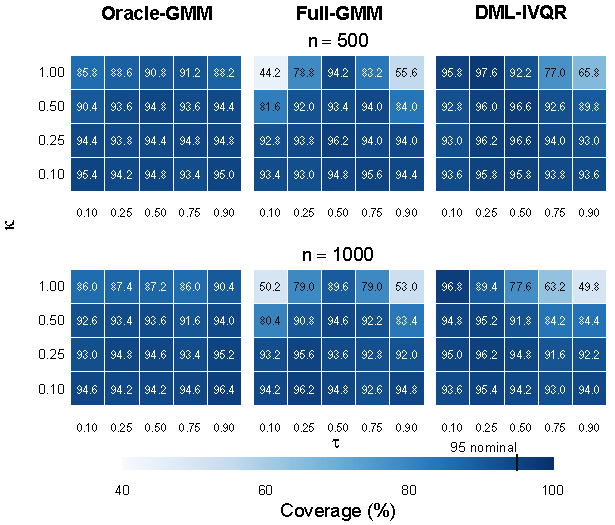
\includegraphics[width=0.72\textwidth]{figures/generated/coverage_heatmap.pdf}
  \caption{Empirical coverage across simulation designs.}
  \label{fig:coverage-heatmap}
  \begin{figurenotes}
    Nominal coverage is 95\%; each cell uses 500 complete replications. Coverage is the fraction of tests accepting the true parameter, evaluated directly at that parameter rather than reconstructed from grid membership. Panel columns identify estimators; panel rows show $n=500$ and $n=1000$. Within each panel, columns show quantiles $\tau$ and rows show relevance $\kappa$, declining from 1.00 to 0.10. Annotations and the common colour scale report percentages. Darker shading indicates higher coverage, not necessarily better calibration.
  \end{figurenotes}
\end{figure}


Increasing the sample size can improve point accuracy without bringing direct-at-truth acceptance closer to the nominal benchmark. At $\kappa=1$, DML truth acceptance falls from $0.976$ to $0.894$ between $n=500$ and $n=1000$ at $\tau=0.25$, from $0.922$ to $0.776$ at $\tau=0.50$, from $0.770$ to $0.632$ at $\tau=0.75$, and from $0.658$ to $0.498$ at $\tau=0.90$. These changes equal $-8.2$, $-14.6$, $-13.8$, and $-16.0$ percentage points. Section~\ref{sec:results-point-accuracy} found lower RMSE at $n=1000$ in all 60 matched comparisons, so lower observed RMSE of the grid minimiser does not imply that direct-at-truth acceptance lies closer to the nominal benchmark.

Direct-at-truth acceptance tends to move toward $0.95$ as relevance weakens, but not monotonically in every cell. Averaged over estimators, quantiles, and sample sizes, truth acceptance rises from $0.798$ at $\kappa=1$ to $0.912$, $0.941$, and $0.944$ as $\kappa$ falls. Only 15 of the 30 estimator--sample-size--quantile sequences are nondecreasing at every step. For example, DML truth acceptance at $n=1000$ and $\tau=0.10$ is $0.968$, $0.948$, $0.950$, and $0.936$ across declining $\kappa$, while Full-GMM truth acceptance at $n=500$ and $\tau=0.25$ is $0.788$, $0.920$, $0.938$, and $0.930$. These reversals are generally small compared with the strong-relevance distortions. Movement toward the nominal acceptance benchmark under weak relevance can accompany less frequent rejection of false candidates; it is not evidence that the reference distribution becomes theoretically justified.

Each rate is based on $R=500$ replications. Under independent replications, its conventional plug-in Monte Carlo standard error is
\[
\operatorname{MCSE}(\widehat p)
=
\sqrt{\frac{\widehat p(1-\widehat p)}{R}}.
\]
The maximum MCSE is approximately $0.022$ and the MCSE at $0.95$ is approximately $0.010$. Appendix~\ref{app:coverage-forensic-audit} strengthens this cell-by-cell uncertainty check. Across 60,000 valid direct-at-truth evaluations, 53 pointwise two-sided 95\% Wilson intervals lie wholly below $0.95$, one lies wholly above it, and 66 contain it. No truth statistic is missing or nonfinite. The intervals use integer acceptance counts without a continuity correction; they are pointwise Monte Carlo intervals, not simultaneous or multiplicity-adjusted tests. An individual rate's MCSE is not used as the standard error of a difference between correlated simulation results. These uncertainty summaries assume independent replications; the historical DML worker-stream independence is not verified (Appendix~\ref{app:evaluation-sequence}).

The audit rules out missing-value handling, nonfinite truth statistics, and reconstruction from rounded grid confidence sets as explanations for the observed below-benchmark truth acceptance. It does not establish invariance to residual-rank arithmetic or numerical solution details; later selected-case audits document such sensitivity, as summarized in Appendix~\ref{app:reproducibility}. It does not isolate a cause among finite-sample approximation error, features of the preserved implementation, or failure of the idealised regularity conditions for the asymptotic chi-square reference law in this DGP. Strong-relevance below-benchmark truth acceptance also shows that weak relevance alone cannot explain the distortions. Direct-at-truth acceptance records retention of the truth; it does not record how readily false candidates are excluded. The next two sections therefore examine power and accepted-set informativeness before interpreting truth acceptance near the nominal benchmark under weak relevance.

The strong-relevance discrepancies are scientifically important because they prevent a simple account in which every departure from a benchmark is attributed to a shortage of excluded signal. They also prevent nominal-looking rates at weaker relevance from being interpreted as validation of the implemented reference law. The saved audit rules out particular reporting explanations but leaves statistical, nuisance and numerical explanations unresolved. The next comparison therefore asks whether candidate retention is accompanied by discrimination against selected false effects, rather than treating movement toward the benchmark as a sufficient improvement.

\subsection{False-Candidate Rejection}
\label{sec:results-power}

Figure~\ref{fig:power-median-combined} reports rejection probabilities at $\tau=0.50$ for candidate values $a_{\Delta}(\tau)=\alpha_0(\tau)+\Delta$. At $\Delta=0$, the candidate is true and rejection probability is labelled empirical size; at each of the six nonzero deviations, it is labelled empirical power against that specified false candidate. The data-generating parameter remains fixed throughout. The plotted probabilities use the same nominal 5\% chi-square cutoff and are not adjusted for differences in empirical size.

\begin{figure}[!htbp]
  \centering
  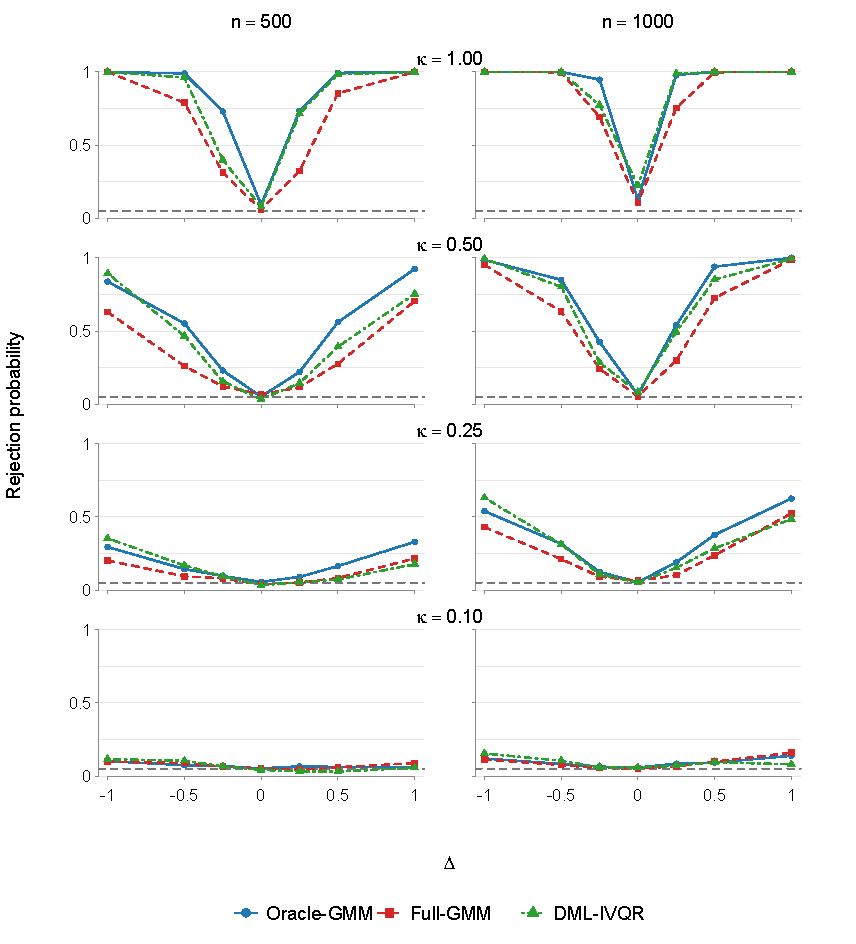
\includegraphics[width=\linewidth]{figures/generated/power_median_combined.pdf}
  \caption{Empirical power at the median.}
  \label{fig:power-median-combined}
  \begin{figurenotes}
    The median benchmark is $\tau=0.50$. Columns show $n=500$ and $n=1000$; rows show $\kappa=1.00,0.50,0.25,0.10$. The horizontal axis is $\Delta=a-\alpha_0(0.50)$, the saved deviation of the tested candidate from truth. Each point uses 500 complete replications and the same nominal 5\% chi-square cutoff; dashed horizontal lines mark 0.05. Rejection at truth is evaluated directly. At $\Delta=0$, rejection probability measures empirical size; at nonzero deviations, it measures power. These rejection probabilities are not size-adjusted. Straight segments are visual guides between evaluated points.
  \end{figurenotes}
\end{figure}


At $n=1000$ and $\Delta=-0.50$, Oracle power falls from $1.000$ through $0.850$ and $0.316$ to $0.082$ as $\kappa$ declines, while DML falls from $1.000$ through $0.802$ and $0.312$ to $0.104$. Full-GMM likewise falls from $0.998$ to $0.076$ between the strongest and weakest settings. For $\Delta=0.50$ at $\kappa=0.25$, power is $0.378$, $0.238$, and $0.286$ for Oracle, Full, and DML, before falling to approximately one tenth for all three at $\kappa=0.10$. The deterioration is therefore already substantial at intermediate relevance, and false effects separated from truth by one half become difficult to exclude in the weakest setting.

Increasing $n$ usually raises power where usable signal remains. At $\kappa=0.50$, Oracle power at $\Delta=-0.50$ rises from $0.552$ to $0.850$, Full from $0.260$ to $0.634$, and DML from $0.466$ to $0.802$ between $n=500$ and $n=1000$. At $\Delta=0.50$, the corresponding changes are $0.560$ to $0.940$, $0.276$ to $0.726$, and $0.392$ to $0.852$. At $\kappa=0.10$, improvements are much smaller and not uniform: Full power at $\Delta=-0.50$ falls from $0.088$ to $0.076$, while DML remains $0.104$; at $\Delta=0.50$, DML rises from $0.030$ to $0.094$. Across all five quantiles and six nonzero deviations, $n=1000$ has higher rejection probability in 305 of 360 matched cells, the same probability in 25, and a lower probability in 30.

The null points clarify why raw power cannot be used as an efficiency ranking. At $n=1000$ and $\kappa=1$, median empirical size is $0.128$ for Oracle, $0.104$ for Full, and $0.224$ for DML, compared with $0.092$, $0.058$, and $0.078$ at $n=500$. DML's strong-relevance rejection of false candidates therefore coexists with the size distortion documented in Section~\ref{sec:results-coverage}. At $n=1000$ and $\kappa=0.10$, empirical sizes are $0.058$, $0.052$, and $0.058$, while power at $\Delta=-0.50$ is only $0.082$, $0.076$, and $0.104$. Rejection of this false candidate is then close to rejection at truth, indicating little discrimination despite approximately nominal size.

The median pattern broadly generalises, but it is not universally monotone. Across all quantiles, sample sizes, estimators, and nonzero deviations, power is nonincreasing as $\kappa$ falls in 162 of 180 sequences. The 18 exceptions are mostly small reversals when rejection is already close to empirical size. Signed differences also occur: for DML at $\tau=0.50$, $n=500$, and $\kappa=0.25$, power is $0.168$ at $\Delta=-0.50$ but $0.072$ at $\Delta=0.50$. Figure~\ref{fig:power-median-combined} displays only $\tau=0.50$, so these full-result counts support generalisation without implying that every quantile follows the plotted paths. The design does not isolate the source of signed asymmetry, and asymmetry in power is not by itself evidence of point-estimation bias.

\FloatBarrier

These rejection frequencies measure how the common reference-cutoff procedure treats specified false candidates in the retained designs. Their scale cannot be interpreted independently of rejection at truth. A procedure with a high null rejection frequency can reject alternatives frequently without providing an equal-size efficiency advantage. Conversely, similarity between truth and false-candidate rejection is evidence of little empirical separation for that alternative, even when truth acceptance looks nominal. The comparison is descriptive and candidate specific; no adjustment of the historical cutoff or reconstruction of size-controlled power is performed.

\subsection{Finite-Grid Informativeness}
\label{sec:results-informativeness}

Figure~\ref{fig:accepted-measure-main} reports the median grid-based accepted-set measure within $A_0=[-1,3]$. The measure increases strictly at every step as $\kappa$ falls in all 30 estimator--sample-size--quantile sequences. At $n=1000$ and $\tau=0.50$, Oracle, Full, and DML medians rise from $0.200$, $0.400$, and $0.300$ at $\kappa=1$ to $3.900$, $3.800$, and $3.900$ at $\kappa=0.10$. Thus lower designed relevance is accompanied by a progressively larger median grid-acceptance measure, even when direct-at-truth acceptance moves closer to $0.95$.

\begin{figure}[!htbp]
  \centering
  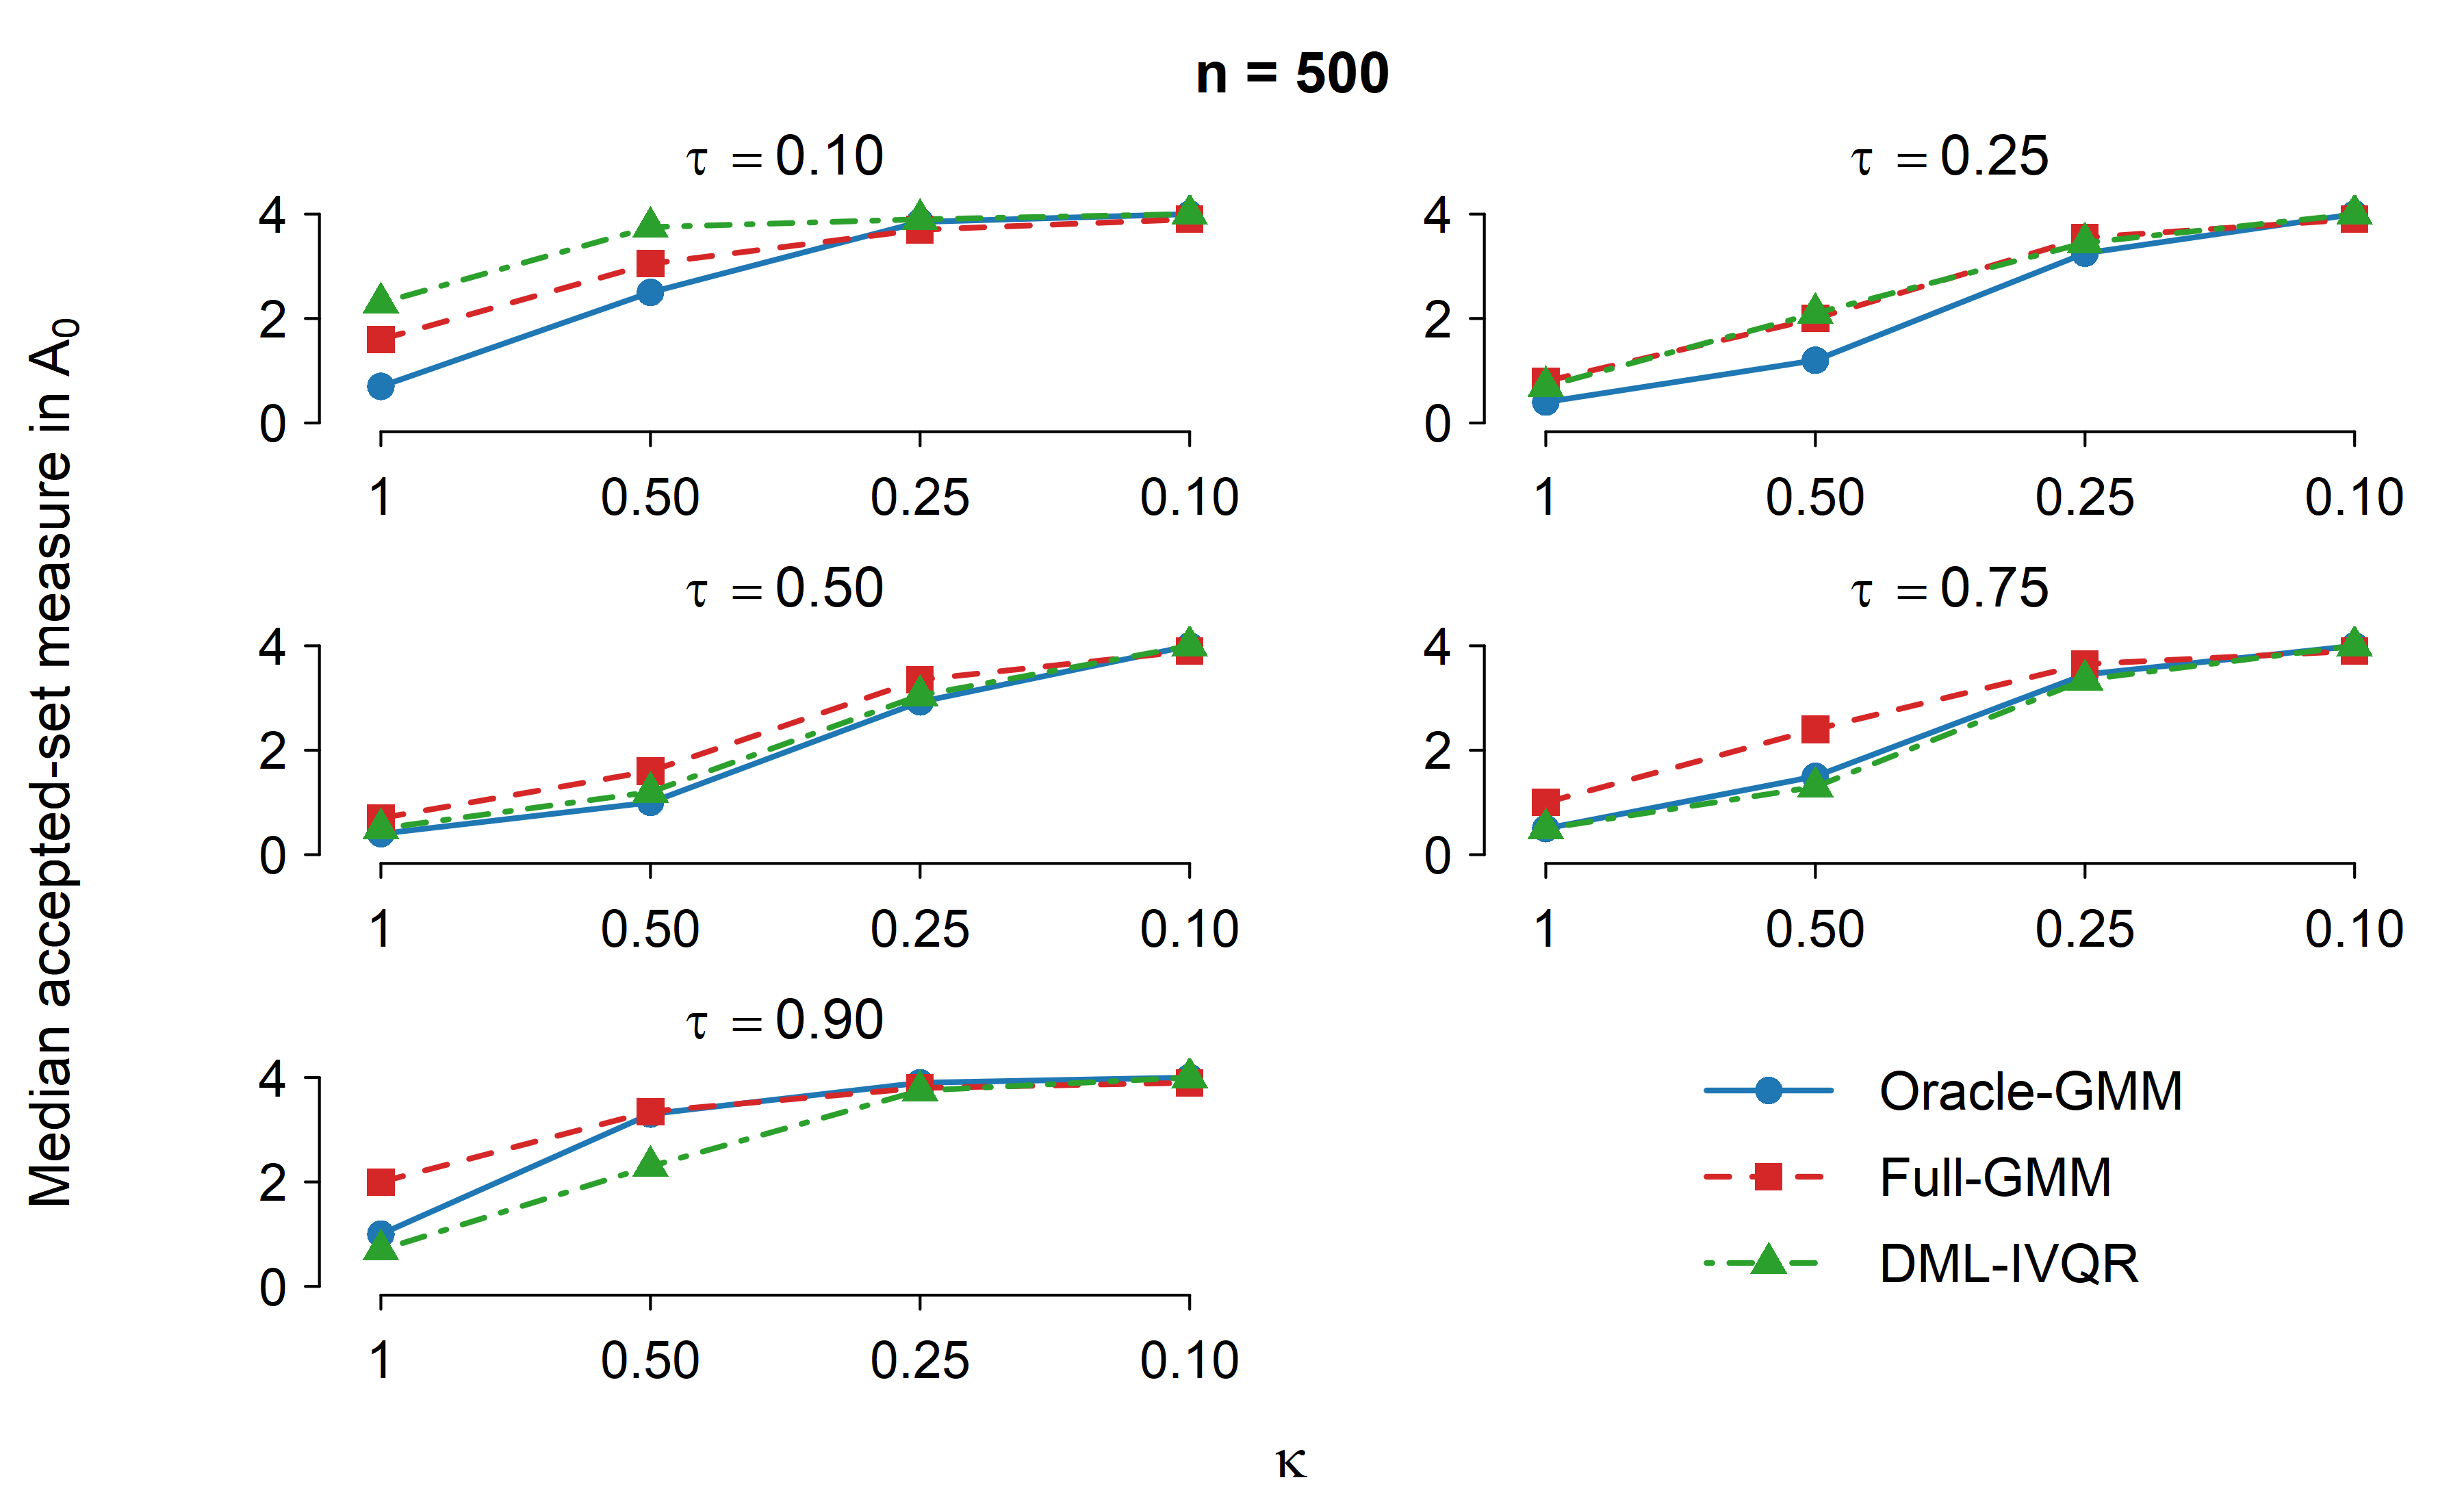
\includegraphics[width=\linewidth]{figures/generated/accepted_measure_n500.png}
  \par\medskip
  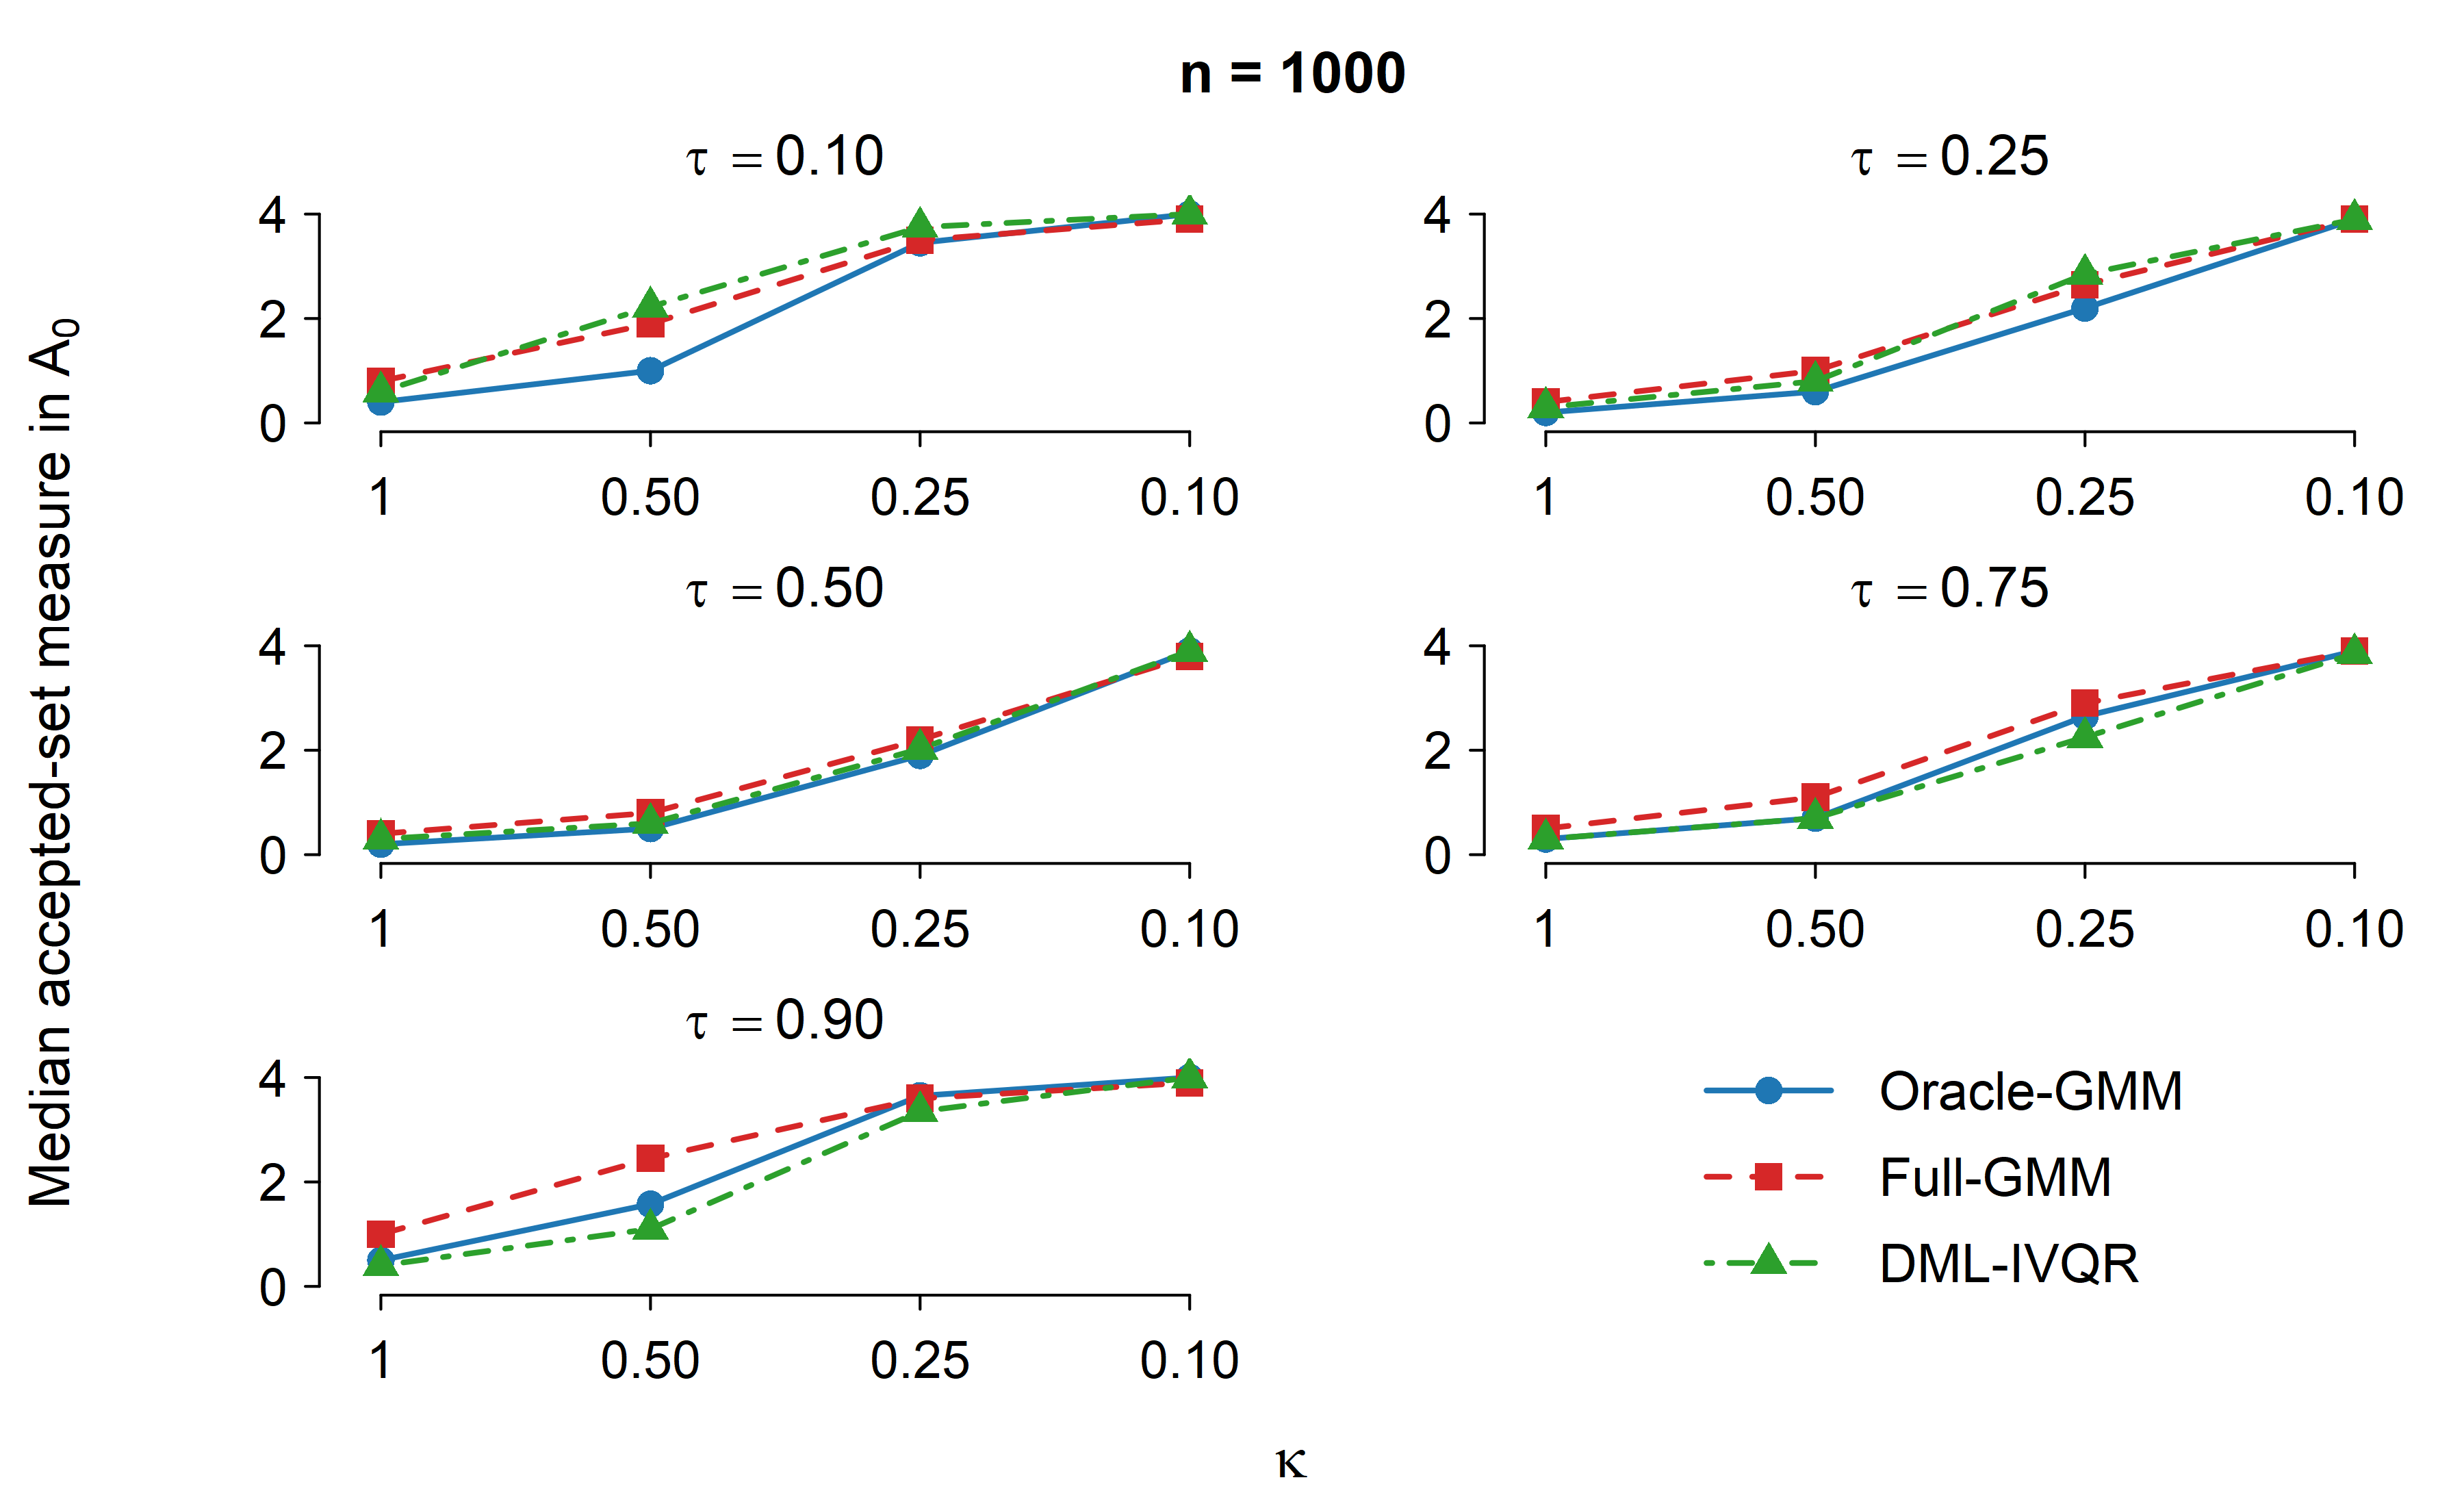
\includegraphics[width=\linewidth]{figures/generated/accepted_measure_n1000.png}
  \caption{Grid-based accepted-set measure within the primary computational domain $A_0=[-1,3]$.}
  \label{fig:accepted-measure-main}

\begin{figurenotes}
Panels show $n=500$ and $n=1000$, using 500 replications per cell. Curves identify Oracle-GMM, Full-GMM, and DML-IVQR; quantile panels show $\tau$. Plotted values are replication medians of the trapezoidal binary-grid-acceptance measure at each $\kappa$. The maximum is four, the width of $A_0$; this is not unrestricted confidence-region length. Lines join evaluated relevance settings as visual guides.
\end{figurenotes}
\end{figure}


Quantile and estimator differences are visible before the weakest setting. At $n=1000$ and $\kappa=0.50$, DML's median measure ranges from $0.600$ at $\tau=0.50$ to $2.225$ at $\tau=0.10$, while Full ranges from $0.800$ to $2.450$ across the five quantiles. Increasing the sample size narrows the median accepted measure in 52 of 60 matched cells and leaves it unchanged in eight; it never widens it. For example, DML at $\tau=0.50$ and $\kappa=0.25$ falls from $3.050$ to $2.025$, whereas at $\kappa=0.10$ it falls only from $4.000$ to $3.900$. The larger sample has a smaller or unchanged observed median accepted measure in these comparisons, with little localization under the weakest relevance setting.

The DML sequence at $n=1000$ and $\tau=0.50$ connects the four inferential summaries. At $\kappa=1$, truth acceptance is $0.776$, the median accepted measure is $0.300$, the full-grid acceptance rate is $0.000$, and power at $\Delta=0.50$ is $1.000$. At $\kappa=0.25$, the corresponding values are $0.948$, $2.025$, $0.040$, and $0.286$. At $\kappa=0.10$, truth acceptance remains near nominal at $0.942$, but the median measure is $3.900$, full-grid acceptance is $0.428$, and power at $\Delta=0.50$ is $0.094$. Truth retention, the amount of the grid retained, acceptance of the entire grid, and rejection of a particular false value therefore answer different questions.

The measure cannot exceed four because it integrates grid acceptance only over $A_0=[-1,3]$. Similar values near four do not imply equivalent unrestricted confidence regions: the calculation does not examine candidates outside $A_0$, and distinct acceptance patterns can produce similar totals. Supplementary Figure~\ref{fig:appendix_full_domain_acceptance} records the frequency with which all 41 evaluated points are accepted. That event does not establish acceptance at every intermediate real value or anywhere outside $A_0$. Direct-at-truth acceptance is also a separate direct evaluation at truth. For DML, fresh pivotal draws mean that direct-truth acceptance and stored-profile acceptance need not coincide even when truth is numerically a grid point.

Appendix~\ref{app:numerical-domain-diagnostics} examines wider domains in a separate diagnostic with $n=1000$, 100 replications, all five quantiles and estimators, $\kappa\in\{1,0.25,0.10\}$, and step $0.1$ on $A_0=[-1,3]$, $A_1=[-3,5]$, and $A_2=[-5,7]$. At $\tau=0.50$ and $\kappa=1$, median DML measure remains $0.300$ on all three domains and $A_2$ boundary acceptance is zero. At $\kappa=0.25$, it grows from $1.950$ to $2.500$ and $3.025$, with $A_2$ boundary acceptance $0.500$. At $\kappa=0.10$, it grows from $3.900$ to $7.500$ and $10.325$, and the $A_2$ boundary is accepted in $0.960$ of usable profiles. Oracle and Full display the same broad weak-relevance pattern, with $A_2$ median measures $11.300$ and $11.450$ and boundary rates $0.830$ and $0.850$ in the corresponding cell.

These domain-expansion values come from a diagnostic run with 100 replications, not the main 500-replication experiment. They show near-stability within the investigated domains under strong relevance and continued failure to localise at intermediate and weak relevance. The diagnostic ends at $A_2$ and does not search the real line. Failure to localise over these domains is evidence of limited numerical informativeness, not proof of global unboundedness or non-identification.

\FloatBarrier

\subsection{Integrated empirical synthesis}
\label{sec:integrated-results}
The most informative comparison combines the directions of change rather than selecting a preferred estimator from a single statistic. The designed relevance ordering is clear, point errors deteriorate as relevance weakens, and the retained sample-size comparison improves RMSE. Yet those gains do not imply movement of direct truth acceptance toward its benchmark, and nominal-looking truth acceptance under weak relevance can coexist with weak discrimination and poor localization. The median DML sequence already reported above makes this disagreement concrete without requiring a new aggregate measure or a recalculation of the frozen results.

Accepted measure near its primary-domain ceiling, frequent full-grid acceptance and low rejection of a specified false value provide different pieces of information. The first describes a quadrature summary, the second a grid-wide event, and the third a separate candidate decision. They do not establish the joint frequency of those features within individual replications. Their comparison nevertheless shows why truth acceptance alone omits an important part of finite-sample performance. The extended-domain diagnostic adds a further boundary: apparent acceptance on a primary grid can remain sensitive to the investigated range, without establishing unrestricted set geometry.

The results therefore support a specific empirical contribution rather than a general inference theorem. Regularized nuisance fitting can coexist with limited candidate discrimination; Oracle knowledge does not prevent the relevance-related deterioration; and strong-relevance distortions require qualifications beyond a weak-signal narrative. Which implementation or regularity feature generates each pattern remains unresolved. Discussion below separates these findings from the mechanism, validity and replay claims that this experiment cannot establish.

\section{Discussion}
\label{sec:results-overall-interpretation}
\subsection{What the controlled relevance comparison establishes}
For the implemented reference-cutoff procedures, reading the diagnostics together identifies weak discrimination and poor localization despite nominal-looking truth acceptance. This is the substantive meaning of the controlled relevance experiment. The compensating-noise construction keeps the documented treatment/endogeneity distribution fixed while changing the excluded signal. Consequently, the observed relevance patterns cannot be explained simply by a changing marginal spread of treatment. This control does not hold the entire observed sample fixed across settings, nor does it isolate the contribution of every computational feature. The experiment studies the complete retained procedures along this particular path.

The scientific value is therefore more specific than showing that weaker instruments make estimation harder. The same design permits apparently reassuring retention of the true candidate to be read alongside limited exclusion of false candidates and extensive acceptance on the maintained grid. These are complementary marginal summaries, not a joint probability, and the false-candidate rates are not size-adjusted comparisons. The controlled construction supports a cleaner description of their disagreement; it does not transform that description into a causal decomposition of nuisance estimation, weak identification and numerical error.

\subsection{Accuracy, retention and discrimination answer different questions}
Point accuracy evaluates the selected grid minimizer, whereas candidate-test behavior concerns the statistic at a specified coefficient. The two summaries use related data but different functionals of the computed profile. A procedure can select a comparatively accurate point while its statistic rejects the true candidate too frequently or retains many false candidates. The sample-size comparisons demonstrate why improving the first summary does not guarantee movement of truth acceptance toward the benchmark. They do not establish a convergence rate, and the available sample sizes cannot identify an asymptotic regime for these implementations.

Truth acceptance is equally incomplete as a description of information. It measures retention at the true effect under the specified reference rule, but does not say how much of the candidate domain is retained. The false-candidate summaries show discrimination at selected deviations, while accepted measure and full-grid frequency describe different aspects of the stored profile. Their combination distinguishes narrow retention around truth from diffuse acceptance across the computational domain. This distinction is useful even when validity is unresolved: the observed decisions remain describable, but a near-benchmark frequency is not promoted to a theorem about coverage.

The interpretation also depends on which inverted object is under discussion. Under a fully specified randomized candidate-test rule, truth acceptance can represent coverage of the corresponding inverted set. That event identity does not establish nominal or uniform validity. Here direct tests are evaluated separately from stored grid profiles, and fresh pivotal draws can differ between calls. Thus the reported direct-at-truth diagnostic is not automatically membership coverage of the separately stored finite-grid set. The Framework makes this distinction explicit; the integrated empirical comparison should not erase it.

\subsection{What the benchmark comparisons reveal}
Oracle-GMM is useful because it knows the designated relevant controls, yet it also loses accuracy and localization as relevance weakens. High-dimensional nuisance estimation is therefore not the sole explanation for deterioration. This comparison does not establish that the oracle implementation is ideal: it still uses the historical density proxy, matrix operations and candidate grid. Knowledge of the relevant controls removes a particular specification burden, not every inferential or computational difficulty. It is a benchmark within the experiment rather than a finite-sample lower bound on error or a certified test.

Likewise, the frequent RMSE advantage of preserved DML-IVQR over preserved Full-GMM does not identify the causal effect of regularization. Their nuisance dimensions, intercept treatment, residualization and fitting routes differ. Quantile-specific reversals remain part of the evidence, rather than exceptions to be discarded. The complete cell evidence is mapped in Appendix~\ref{app:evidence-map}. A controlled component comparison would require changing and documenting individual features in a separately specified study; that experiment has not been carried out here. No ranking of the retained implementations should be extended to all DGPs or all high-dimensional IVQR methods.

\subsection{Theoretical motivation and executable limitations}
Orthogonalization can reduce local sensitivity to nuisance errors under its conditions, but it cannot create the treatment--instrument information needed to distinguish structural candidates \parencite{chernozhukov_et_al_2018}. Identification-robust inference concerns validity under a procedure's own assumptions, not guaranteed discrimination \parencite{chernozhukov_hansen_2008,jun_2008}. These concepts explain the questions asked by the experiment. They do not certify that the preserved density proxy, projection and same-sample nuisance estimates satisfy the ideal score's conditions.

The retained mixed-density argument is especially important for that boundary. It concerns the residual density after integrating over treatment, not the density conditional on a realized positive treatment value and not the fitted-normal proxy. Its divergence blocks the displayed standard finite-density justification. It does not identify an alternative limiting distribution, prove that all possible inferential arguments fail, or make the recorded statistics mathematically meaningless. The implementation differences and selected numerical sensitivities were not varied independently to identify the source of a particular acceptance or rejection pattern. Missing cross-fitting alone is not such a diagnosis either.

Numerical certificates have a similarly specific role. The later investigations concern fixed objectives and exported inputs within selected cases. They document residual-rank and decision sensitivity and do not replace the historical Monte Carlo fits. A certificate for a specified problem is not a full-experiment error frequency, and improved objective accuracy need not imply identical residual signs or test decisions. Historical worker-specific penalty states and portable runtime reproduction also remain incomplete. Inspection of frozen evidence must therefore be distinguished from deterministic reporting, selected-case replay and exact historical stochastic replay.

\subsection{Finite domains and reporting implications}
Finite-grid accepted measure summarizes recorded binary decisions, rather than continuous boundaries. Full-grid acceptance is a different event, and expansion to a wider finite domain is a localization diagnostic rather than a search of the real line. Similar accepted measures can arise from different patterns of retained candidates; a nonaccepted boundary cannot rule out a disconnected component farther away. The preserved domain diagnostics are informative about these computational limits without establishing global boundedness, unboundedness or formal nonidentification.

For future Monte Carlo reporting, this study supports stating the decision rule, candidate domain and evaluation sequence alongside point-error summaries. It also motivates distinguishing raw false-candidate rejection from comparisons between tests of equal size. These are reporting implications drawn from this experiment, not a recommendation that a particular estimator or correction is universally preferable. Further comparisons would need their own DGPs, nuisance assumptions and randomization specifications. Within the present evidence, the defensible conclusion is that accuracy, truth retention and localization must be read together before a favourable summary is interpreted as informative inference.

\section{Conclusion}
This study asks how weakening excluded-instrument relevance changes the finite-sample behavior of preserved high-dimensional IVQR procedures when the documented treatment/endogeneity distribution is held fixed. The question is narrower than whether IVQR can accommodate endogeneity or whether orthogonal scores can support inference under suitable assumptions. Those are questions addressed by the motivating literature. The present contribution is a controlled empirical comparison that traces the relationship among point accuracy, retention of the true candidate, rejection of specified false candidates and localization of the accepted numerical profile. It extends the fixed-relevance simulation of \textcite{chen_huang_tien_2021} without introducing a new estimator or asymptotic theorem.

The experimental construction reduces the excluded signal and adds independent compensating noise under the stated Gaussian assumptions. This preserves the documented joint treatment/outcome-disturbance distribution and the structural effects while changing treatment--instrument relationships. It avoids interpreting a simultaneous change in treatment dispersion as a consequence of relevance alone. The construction does not preserve each realized treatment or outcome across settings, and the relevance parameter is not a universal measure of quantile-specific identification. Its usefulness lies in making a particular comparison explicit and interpretable, rather than in defining a general weak-instrument classification for IVQR applications.

The central empirical result is disagreement among measures that can each appear reassuring in isolation. As relevance weakens, truth acceptance can approach the nominal benchmark while false-candidate rejection becomes limited and the maintained grid retains little localization. The point-error comparisons provide a second warning: lower RMSE at the larger sample size does not imply that truth acceptance moves closer to its benchmark. Strong-relevance distortions and quantile asymmetries remain important counterpoints, showing that weak relevance alone cannot account for all observed patterns. The contribution is the documented configuration of these findings in the controlled experiment, rather than the general observation that weak identification can reduce power.

The benchmark comparisons sharpen that interpretation without identifying its mechanism. Oracle-GMM also deteriorates despite knowing the designated relevant controls, so high-dimensional nuisance estimation cannot be the sole explanation for the loss of performance. DML-IVQR often has smaller point errors than Full-GMM, but the retained exceptions and differences in nuisance dimension, residualization and fitting conventions prevent a universal ranking or an attribution to regularization alone. The comparison concerns complete historical implementations. It does not estimate the effect of switching a single computational component, and it supplies no evidence about methods or DGPs that were not included.

The inferential objects must also remain distinct. A direct-at-truth evaluation describes a candidate decision under the implemented reference cutoff. For a coherently specified randomized test and its inversion, that acceptance event can represent membership of truth in the conceptual inverted set; the identity alone says nothing about attainment of a nominal level. The stored finite-grid accepted set in this experiment is evaluated separately, and fresh pivotal penalties can distinguish direct and stored-profile decisions. Raw false-candidate rejection is not a size-adjusted power comparison. Neither high truth acceptance nor a compact accepted profile establishes theoretically valid confidence-set coverage for the implemented procedures.

Several limitations qualify the theoretical interpretation. The non-finite mixed residual density prevents use of the displayed standard finite-density argument, while the historical code uses a different fitted-normal proxy. Same-sample nuisance estimation, intercept and projection conventions, penalty randomness and finite solver outputs remain features of the objects being compared. No separate experiment isolates their contributions to the rejection patterns. The selected numerical audits document rank and decision sensitivity for specified problems but do not certify every historical decision or a full-experiment error frequency. These qualifications restrict inference claims without invalidating the descriptive content of the frozen numerical records.

The computational domain creates an additional limit. Accepted measure and full-grid frequency describe the investigated grid, not continuous boundaries or unrestricted set geometry. Wider-domain diagnostics reveal how much localization changes over the examined ranges, but do not establish global boundedness or nonidentification. Exact historical stochastic replay is also not established from the parent seed: worker-specific penalty streams and portable installation details are incomplete. These limits explain why evidence inspection, reporting from frozen outputs and numerical replay should be described separately. A transparent computational account is part of interpreting the experiment, not a substitute for an inference argument.

Three concrete research directions follow, without being carried out in this revision. First, a separately specified design with an analytically checked finite mixed density could distinguish the relevance comparison from this particular regularity limitation while preserving clearly stated distributional controls. Second, a component comparison could vary nuisance fitting, residualization, density treatment or cross-fitting under a prespecified randomization scheme, allowing mechanisms that are confounded here to be examined separately. Third, a domain and computation study could predefine wider candidate searches and archive worker states and candidate-level inputs, distinguishing numerical decision stability from inferential calibration. Each would create new evidence and would require its own scientific justification; none retrospectively repairs the present archive.

The immediate scientific implication is therefore one of interpretation. In a simulation of an implemented IVQR procedure, point accuracy, truth acceptance and the ability to exclude alternatives are distinct properties. Reporting them together can expose weak discrimination and poor localization that a single performance measure conceals. Within the studied designs, this controlled comparison provides such evidence while leaving the theoretical validity and causal source of the observed decision patterns unestablished. That combination of substantive findings and explicit limits is the contribution of the article.

\label{w3:main-end}
\section*{Declarations}
\paragraph{Funding.} This research received no external funding.

\paragraph{Competing interests.} The authors declare no financial or non-financial conflicts of interest.

\paragraph{Author contributions.} Both authors contributed equally.

\paragraph{AI assistance.} AI tools assisted with grammar checking, linguistic editing, and manuscript documentation.

\paragraph{Ethics and informed consent.} The study uses simulated data without human participants or personal data. Ethics approval and informed consent were not required.

\section*{Data and code availability}
\ifdefined\WfourAnonymous
\WfourRepository
\else
The research code and archived simulation results are maintained at \url{https://github.com/U-Olim/IVQR-Under-the-Weak-Instruments.git}. The repository supports verification of reported results from archived outputs; exact historical stochastic replay is not established.
\fi

\FloatBarrier
\par\vspace{3\baselineskip}
\label{w3:references-start}
\begingroup
\defbibheading{bibliography}[References]{\noindent{\normalfont\Large\bfseries #1}\par\nobreak\vspace{\baselineskip}}
\printbibliography[title={References}]
\endgroup
\clearpage
\appendix
\label{w3:appendices-start}
\section*{Online supplementary material}
\noindent Appendices A--D provide numerical-domain diagnostics, the controlled-design derivation, the coverage audit, and implementation notes. They are included here to keep all cross-references resolvable in a single review PDF.
\renewcommand{\theequation}{\thesection.\arabic{equation}}
\renewcommand{\thetable}{\thesection.\arabic{table}}
\renewcommand{\thefigure}{\thesection.\arabic{figure}}
\renewcommand{\theHequation}{\thesection.\arabic{equation}}
\renewcommand{\theHtable}{\thesection.\arabic{table}}
\renewcommand{\theHfigure}{\thesection.\arabic{figure}}
\section{Numerical-Domain Diagnostics}
\setcounter{equation}{0}\setcounter{table}{0}\setcounter{figure}{0}
\label{app:numerical-domain-diagnostics}

\label{app:domain-choice}

The primary computational domain is \(A_0=[-1,3]\), evaluated on 41 equally spaced candidate values with step size \(h=0.1\). 
Using the same domain for all sample sizes, quantiles, instrument-relevance settings, and estimators makes the accepted-set measures directly comparable across the simulation design.

The interval also contains the true structural quantile effects for all five investigated quantiles. Under the data-generating process,
\[
\alpha_0(\tau)=1+\Phi^{-1}(\tau),
\]
so the true effects are approximately \(-0.282\), \(0.326\), \(1.000\), \(1.674\), and \(2.282\) for \(\tau=0.10,0.25,0.50,0.75,\) and \(0.90\), respectively. All five structural truths lie strictly inside \(A_0\); using their unrounded values, the minimum distance to either endpoint is approximately \(0.718\). The interval should therefore be understood as a common numerical search domain, not as an assumed theoretical parameter space.

A finite search domain can nevertheless become restrictive when instruments are weak and many candidate values are accepted. For this reason, a separate sensitivity diagnostic expands the search range from \(A_0=[-1,3]\) to \(A_1=[-3,5]\) and then to \(A_2=[-5,7]\). Under strong instrument relevance, expanding the domain adds little accepted measure, indicating that accepted grid values are well localized within the investigated ranges, without establishing continuous accepted components. At intermediate relevance, the wider domains contain additional accepted values in some profiles. Under the weakest relevance setting, the accepted measure continues to increase as the domain is expanded and does not stabilize within \(A_2\).

These results clarify the interpretation of the main accepted-set measure. A value close to four in \(A_0\) means that the trapezoidal grid-acceptance summary is close to its maximum on the four-unit primary domain; it does not establish acceptance between evaluated points or unrestricted confidence-region length. Similarly, continued acceptance in the wider domains indicates poor numerical localization over the ranges examined, but it does not by itself establish that the theoretical confidence region is globally unbounded or that identification completely fails.

Table~\ref{tab:appendix-grid-measures} reports representative median-quantile comparisons for all three estimators, transcribed from the frozen diagnostic; Figure~\ref{fig:grid-domain} retains the expansion pattern across quantiles.

The diagnostic contains one singular-design error: replication 35, $\tau=0.90$, $\kappa=0.10$, DML-IVQR, candidate $a=-2.1$ in Stage 1. Stage 2 adds no new evaluation errors. Incomplete profiles receive missing aggregate measures: the affected expanded-domain cell uses 99 usable replications; other cells use 100. The representative cells below each use 100 complete profiles. A nonaccepted boundary does not rule out disconnected accepted components beyond the examined interval. The full five-table diagnostic remains in the preserved W3 source, outside this shortened manuscript.
\begin{table}[htbp]
\centering
\caption{Representative domain expansion: median grid-accepted measure at $n=1000$, $\tau=0.50$.}
\label{tab:appendix-grid-measures}
\begin{tabular}{clrrr}
\toprule
$\kappa$ & Estimator & $A_0$ & $A_1$ & $A_2$ \\
\midrule
1.00 & Oracle-GMM & 0.200 & 0.200 & 0.200 \\
1.00 & Full-GMM & 0.400 & 0.400 & 0.400 \\
1.00 & DML-IVQR & 0.300 & 0.300 & 0.300 \\
0.25 & Oracle-GMM & 1.875 & 2.200 & 2.200 \\
0.25 & Full-GMM & 2.250 & 2.400 & 2.550 \\
0.25 & DML-IVQR & 1.950 & 2.500 & 3.025 \\
0.10 & Oracle-GMM & 3.825 & 7.600 & 11.300 \\
0.10 & Full-GMM & 3.900 & 7.625 & 11.450 \\
0.10 & DML-IVQR & 3.900 & 7.500 & 10.325 \\
\bottomrule
\end{tabular}
\begin{tablenotes}
Frozen values for strong ($\kappa=1$), intermediate ($0.25$), and weak ($0.10$) relevance; 100 complete profiles per row. Domains are $A_0=[-1,3]$, $A_1=[-3,5]$, $A_2=[-5,7]$, with spacing 0.1. The measure summarizes evaluated grid points by trapezoidal quadrature; it is not unrestricted confidence-region length. This representative subset does not replace the across-quantile figure or establish global boundedness.
\end{tablenotes}
\end{table}

\begin{figure}[!t]
  \centering
  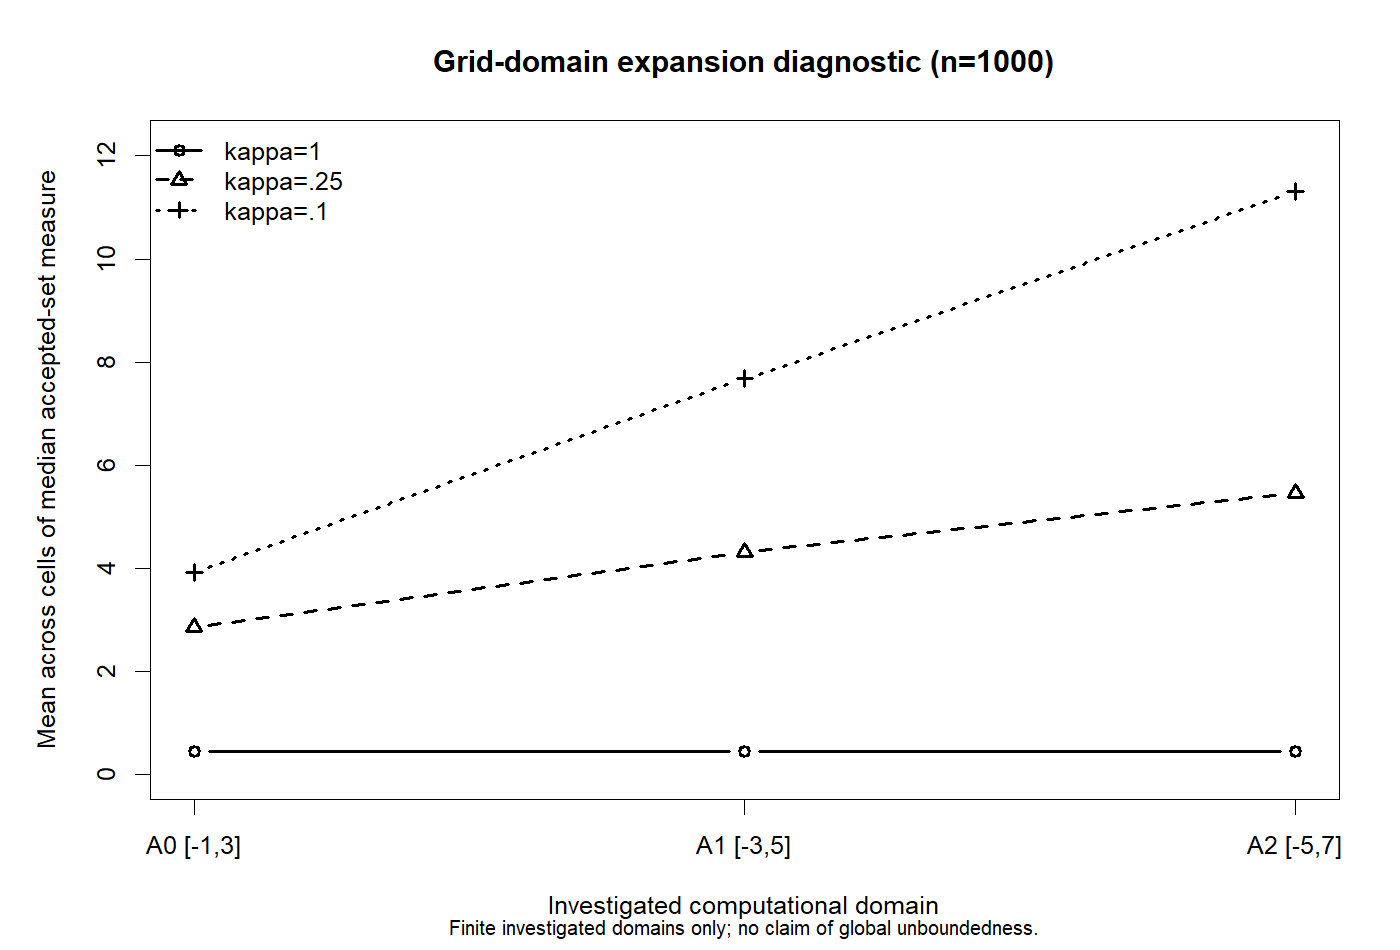
\includegraphics[width=0.72\textwidth]{figures/grid_domain_expansion.png}
  \caption{Sensitivity of the accepted set to expansion of the computational domain}
  \label{fig:grid-domain}
  \begin{figurenotes}[Note]
    Each plotted value is the mean across 15 estimator--quantile cells of the cell-specific median accepted-set measure for the stated $\kappa$ and domain. The investigated domains are $A_0=[-1,3]$, $A_1=[-3,5]$, and $A_2=[-5,7]$. The diagnostic records whether the accepted set stabilizes within these numerical domains; it does not establish global boundedness or unboundedness.
  \end{figurenotes}
\end{figure}

\FloatBarrier

Figure~\ref{fig:appendix_full_domain_acceptance} in Appendix~\ref{app:coverage-forensic-audit} complements these expansion diagnostics by reporting how often all candidates within the primary grid are accepted.
\Needspace{7\baselinedist}

\clearpage
\section{Derivation and Properties of the \texorpdfstring{$\kappa$}{kappa} Extension}
\label{app:kappa-derivation}
\setcounter{equation}{0}\setcounter{table}{0}\setcounter{figure}{0}
The extension changes assignment while retaining the baseline primitives in Section~\ref{sec:monte-carlo-design}. The excluded sum has variance two, $\epsilon_i$ has variance one, and $\operatorname{Cov}(u_i,\epsilon_i)=0.3$. Introduce independent $w_i\sim\mathcal N(0,1)$ and write
\begin{equation}
 d_i^*(\kappa)=\kappa(z_{1i}+z_{2i})+c(\kappa)w_i+\epsilon_i,
 \qquad \kappa\in[0,1].
 \label{eq:appendix-kappa-unknown}
\end{equation}
Independence eliminates all cross-covariances between index components. Preserving the baseline variance requires
\[
2\kappa^2+c(\kappa)^2+1=3,
\qquad c(\kappa)=\sqrt{2(1-\kappa^2)},\quad 0\le\kappa\le1.
\]
The nonnegative root is conventional; normal symmetry makes its sign distributionally immaterial. This coefficient is specific to the independent-noise construction.
\begin{equation}
 \begin{aligned}
 d_i^*(\kappa)&=\kappa(z_{1i}+z_{2i})+\sqrt{2(1-\kappa^2)}\,w_i+\epsilon_i,\\
 D_i(\kappa)&=\Phi\!\left(d_i^*(\kappa)\right).
 \end{aligned}
 \label{eq:appendix-kappa-assignment}
\end{equation}
Normality gives $d_i^*(\kappa)\sim\mathcal N(0,3)$, where 3 denotes variance. Thus for $0<d<1$,
\begin{equation}
 \begin{aligned}
 \Pr\!\left[D_i(\kappa)\le d\right]
 &=\Pr\!\left[\Phi(d_i^*(\kappa))\le d\right]\\
 &=\Pr\!\left[d_i^*(\kappa)\le\Phi^{-1}(d)\right]\\
 &=\Phi\!\left(\frac{\Phi^{-1}(d)}{\sqrt{3}}\right).
 \end{aligned}
 \label{eq:appendix-treatment-cdf}
\end{equation}
The CDF is zero below zero and one above one. It is independent of $\kappa$, but is not Uniform$(0,1)$. Equal variance establishes this invariance because the index is normal, not for arbitrary distributions.

Write $Z_{ji}=z_{ji}+v_{ji}+C_{ji}$, where $C_{1i}=X_{2i}+X_{3i}+X_{4i}$ and $C_{2i}=X_{7i}+X_{8i}+X_{9i}+X_{10i}$. Independence yields
\[
\operatorname{Cov}(Z_{ji},d_i^*(\kappa))
=\kappa\operatorname{Cov}(z_{ji},z_{1i}+z_{2i})=\kappa,
\qquad j=1,2.
\]
This latent-index covariance is not $\operatorname{Cov}(Z_{ji},D_i(\kappa))$ or a formal IVQR identification statistic.

Similarly, $\operatorname{Cov}(u_i,d_i^*(\kappa))=\operatorname{Cov}(u_i,\epsilon_i)=0.3$. Joint normality gives
\begin{equation}
 \begin{pmatrix}u_i\\d_i^*(\kappa)\end{pmatrix}
 \sim\mathcal{N}\!\left(
 \begin{pmatrix}0\\0\end{pmatrix},
 \begin{pmatrix}1&0.3\\0.3&3\end{pmatrix}\right).
 \label{eq:appendix-endogeneity-invariance}
\end{equation}
The invariant mean vector and covariance matrix establish invariance of the entire joint distribution, hence of $(u_i,\Phi(d_i^*(\kappa)))$. Covariance alone would not suffice without joint normality. Individual treatment realizations can differ across relevance settings.

At fixed $d>0$, $Y_i(d)=1+5\sum_{j=1}^7X_{ji}+d(1+u_i)$. Independence of $u_i$ and $X_i$ gives $Q_{Y_i(d)\mid X_i}(\tau)=1+5\sum_{j=1}^7X_{ji}+d[1+\Phi^{-1}(\tau)]$. The unchanged potential-outcome equation therefore preserves $\alpha_0(\tau)$. This is a structural quantile at fixed treatment, not an observational conditional quantile at realized endogenous treatment.

The endpoints recover the baseline ($\kappa=1$) or remove the excluded primitive signal ($\kappa=0$); the weakest simulated setting remains positive. These are construction-specific properties, not global IVQR identification results.

Table~\ref{tab:kappa-illustration} records the analytical variance allocation for all simulated settings.
\begin{table}[!htbp]
\caption{Variance allocation in the $\kappa$-extension.}
\label{tab:kappa-illustration}
\centering
\begin{tabular}{rrrrr}
\toprule
$\kappa$ & \shortstack{Coefficient\\$\sqrt{2(1-\kappa^2)}$} & \shortstack{Signal variance\\$2\kappa^2$} & \shortstack{Noise variance\\$2(1-\kappa^2)$} & \shortstack{Total index\\variance} \\
\midrule
1.00 & 0.0000 & 2.0000 & 0.0000 & 3.0000 \\
0.50 & 1.2247 & 0.5000 & 1.5000 & 3.0000 \\
0.25 & 1.3693 & 0.1250 & 1.8750 & 3.0000 \\
0.10 & 1.4071 & 0.0200 & 1.9800 & 3.0000 \\
\bottomrule
\end{tabular}
\begin{tablenotes}
Values are calculated directly from the construction, not simulated. The disturbance $\epsilon_i$ contributes the remaining variance of one in every row.
\end{tablenotes}
\end{table}

\FloatBarrier

\section{Coverage Audit and Inferential Informativeness}
\setcounter{equation}{0}\setcounter{table}{0}\setcounter{figure}{0}
\label{app:coverage-forensic-audit}
The frozen audit covers 60,000 direct tests at the exact structural truth: 500 replications in each of 120 sample-size, quantile, relevance and estimator cells. No true-parameter $W$ statistics are missing or nonfinite. Of the pointwise 95\% Wilson intervals, 53 lie below 0.95, one lies above it, and 66 contain it (Table~\ref{tab:coverage-audit-summary}). The comparisons use unrounded endpoints; these are Monte Carlo uncertainty intervals without multiplicity adjustment. A rate's Monte Carlo standard error is not a standard error for a difference between correlated results. The audit rules out missing-value handling and plotting-grid artifacts as explanations for these discrepancies; it does not establish nominal calibration or validate the reference distribution.

\begin{table}[!ht]
\caption{Direct-at-truth coverage audit.}
\label{tab:coverage-audit-summary}
\centering
\begin{tabular}{lrrrrrrr}
\toprule
Estimator & $n$ & Cells & \shortstack{Coverage\\min.} & \shortstack{Coverage\\max.} & \shortstack{Upper\\$<0.95$} & \shortstack{Lower\\$>0.95$} & \shortstack{Missing/\\nonfinite} \\
\midrule
Oracle-GMM & 500 & 20 & 0.858 & 0.954 & 6 & 0 & 0 \\
Oracle-GMM & 1000 & 20 & 0.860 & 0.964 & 8 & 0 & 0 \\
Full-GMM & 500 & 20 & 0.442 & 0.962 & 9 & 0 & 0 \\
Full-GMM & 1000 & 20 & 0.502 & 0.962 & 12 & 0 & 0 \\
DML-IVQR & 500 & 20 & 0.658 & 0.976 & 8 & 1 & 0 \\
DML-IVQR & 1000 & 20 & 0.498 & 0.968 & 10 & 0 & 0 \\
\bottomrule
\end{tabular}
\begin{tablenotes}
Each row covers 20 quantile--$\kappa$ cells, with 500 direct-at-truth evaluations per cell. Coverage is reported as a proportion. The upper/lower columns count cells whose unrounded Wilson upper endpoint is below 0.95 or lower endpoint is above 0.95. Intervals use integer acceptance counts, the verified denominator, and the two-sided 95\% Wilson formula without continuity correction. They are pointwise Monte Carlo intervals, not simultaneous or multiple-testing-adjusted intervals; exclusion counts are descriptive audit summaries. Missing/nonfinite counts concern direct-at-truth $W$ evaluations (missing values are counted once).
\end{tablenotes}
\end{table}

\FloatBarrier
Direct truth acceptance is a separate candidate evaluation, not membership coverage of the stored finite-grid accepted set. Fresh pivotal draws in DML-IVQR can make these events differ even when truth is a grid point. Figure~\ref{fig:appendix_full_domain_acceptance} uses stored profiles to report acceptance of all 41 points in $A_0=[-1,3]$. Nominal-looking truth acceptance can coexist with little exclusion of false effects. All-grid acceptance establishes neither acceptance between evaluated points nor acceptance of the real line. Appendix~\ref{app:numerical-domain-diagnostics} addresses expansion over finite investigated domains.
\begin{figure}[!ht]
  \centering
  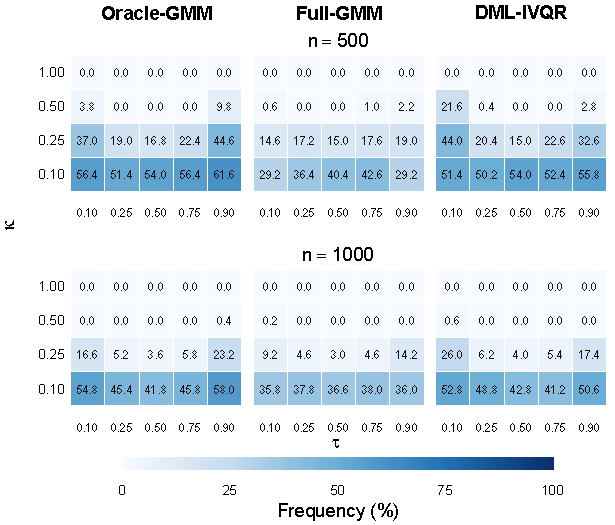
\includegraphics[width=0.72\textwidth]{figures/generated/full_domain_acceptance_heatmap.pdf}
  \caption{Full-domain grid acceptance frequencies.}
  \label{fig:appendix_full_domain_acceptance}
  \begin{figurenotes}
    Each cell reports the percentage of 500 complete replications accepting all 41 evaluated grid points in $A_0=[-1,3]$, with step size $h=0.1$. Panel columns identify estimators; panel rows show $n=500$ and $n=1000$. Within each panel, columns show quantiles $\tau$ and rows show relevance $\kappa$, declining from 1.00 to 0.10. Darker shading on the shared 0--100\% scale means more frequent full-domain grid acceptance. This event neither denotes acceptance of the entire real line nor establishes an unbounded unrestricted confidence region.
  \end{figurenotes}
\end{figure}

\FloatBarrier
\clearpage

\section{Reproducibility and Implementation Notes}
\label{app:reproducibility}
\setcounter{equation}{0}\setcounter{table}{0}\setcounter{figure}{0}
\subsection{Archive and reproducibility boundaries}
\label{app:evidence-map}
\WfourRepository
The evidence map is: relevance, \path{code/data/kappa_strength_summary.csv}; complete cell summaries, direct truth statistics and grid profiles, \path{code/results/main/n500/} and \path{code/results/main/n1000/}; false-candidate rejection, their \path{power_summary.csv} and compressed replication records; expanded-domain summaries and selected numerical comparisons, \path{code/results/diagnostics/}. The abstract's $0.942/3.900/0.094$ contrast uses direct truth acceptance, median grid-accepted measure and rejection at offset $+0.50$, respectively, for DML-IVQR at $n=1000$, $\tau=0.50$, $\kappa=0.10$; it is not a joint event or validated grid-set coverage. Historical file inventories are retained separately from the manuscript.
The selected package contains preserved scientific modules in \path{code/src/}, configuration and historical version records in \path{code/config/}, main outputs in \path{code/results/main/}, and diagnostic summaries in \path{code/results/diagnostics/}. The original environment is Windows R~3.4.3 with five workers, \texttt{quantreg}~5.34 and \texttt{hdm}~0.2.0; full version inventories and reporting instructions accompany the package rather than the manuscript. Main outputs remain frozen. Deterministic inspection of saved records differs from historical stochastic replay: worker-specific RNG streams and full main-run penalty states were not archived. Parent seed 675 alone does not establish replay or worker-stream independence. Large expanded-grid profiles, saved primitives and a portable historical runtime are not established as publicly deposited. The historical freeze identifier \texttt{ac9a9cca} remains unresolved and is not a verified release checkout.

Selected-case numerical audits found five Policy A/C decision differences among 24 saved candidate problems. Policy C retains the density/projection pathway but uses exact outcome residual ranks. These panels do not estimate an experiment-wide error rate or replace any historical results. Certificates concern fixed objectives and stated inputs, not every historical decision or adaptive calibration trajectory. Rights and both-author distribution approval remain unresolved; authenticated repository access does not establish anonymous public access or permission to redistribute.

\subsection{Historical evaluation sequence}
\label{app:evaluation-sequence}
One historical replication proceeds as follows.
\begin{enumerate}
\item Generate one set of primitives; construct a sample at each relevance setting. Within that setting all three estimators share $(Y,D,X,Z)$. Reusing primitives across settings does not hold realized $(Y,D)$ fixed.
\item For each quantile and estimator, profile the ordered 41-point primary grid. At each DML candidate $a$, call \texttt{lambda\_BC\_author} afresh (1000 artificial uniform columns), then fit \texttt{quantreg::rq(y-a*D\string~X, method="lasso")} with the resulting penalty and an intercept. Refit nuisances at each candidate; there is no post-Lasso refit. Oracle and Full instead call unpenalized \texttt{quantreg::rq} with their designated controls.
\item Form candidate outcome residuals and the proxy \texttt{dnorm(e, mean(e), var(e))}. Residualize instruments using the DML transformed regressions or benchmark matrix rule below; numerical termination and last-used penalty conventions are specified once in Appendix~\ref{app:finite-solvers}.
\item Apply the literal computed-residual rule $r_i=\mathbf1\{\widehat e_i\leq0\}$, with no residual tolerance. Set $s_i=\tau-r_i$, $g=\sum_i\widehat\Psi_i s_i$ and $S=\sum_i\widehat\Psi_i\widehat\Psi_i' s_i^2$. The statistic is $g'S^{-1}g$, equivalent to the normalized definition in Section~\ref{sec:framework}. Use direct \texttt{solve} and the retained nominal chi-square cutoff; singular or non-finite evaluations are failures, not acceptances.
\item Retain the first grid minimum for the point estimate and the stored grid decisions for informativeness summaries. After profiling, separately evaluate the true effect and six specified false candidates. DML again invokes its candidate routine, with fresh pivotal draws, in a separate five-worker evaluation. Direct-at-truth acceptance and false-candidate rejection therefore do not reuse stored grid statistics, even when candidates coincide. Failed profiles receive no point estimate; the documented failure conventions remain in force.
\end{enumerate}
The archived estimator includes both sample randomness and algorithmic penalty randomness. Common observed data do not imply common pivotal draws across estimators, candidates, or repeated calls. Worker-specific RNG stream assignments and the full main-run candidate penalty states were not archived as a replay specification; seed 675 alone neither reproduces every historical penalty nor establishes independence of worker streams. Saved Stage 2G cases with exported states have a narrower replay scope. The conventional Monte Carlo standard-error summaries do not verify historical stream independence. Frozen CSV inspection and selection of existing table/figure assets require no stochastic rerun; they do not recover missing RNG states.

\subsection{Penalty, density proxy, and residualization}
\label{app:penalty-implementation}
For each candidate, $b_0$ is the fitted outcome intercept and $b$ the slopes. In the preserved \texttt{rq.fit.lasso} augmented-observation implementation, the unscaled check-loss sum receives a penalty with factor $1/2$. The vector $\lambda^{rq}(a)$ is the supplied routine argument, including an intercept penalty. There is no post-Lasso refit. Let $s_k=(n^{-1}\sum_iX_{ik}^2)^{1/2}$; $U_{ir}$ are independent artificial Uniform$(0,1)$ draws, with $r=1,\ldots,1000$, and $\widehat Q_{0.9}$ is their empirical pivotal-statistic 90th percentile. Fresh draws are made on every penalty call. This is algorithmic randomness, not sample splitting.

In the following formulas, $\phi(e;\mu,\sigma)$ denotes a normal density parameterized by standard deviation. The proxy supplies $\widehat\sigma_\epsilon^2$ in that argument: the preserved R call is \texttt{dnorm(e, mean(e), var(e))}. It evaluates a fitted-normal density at residuals rather than estimating the theoretical conditional density at zero. The sample-variance convention is
\[
 \widehat\sigma_\epsilon^2(a)=\frac{1}{n-1}\sum_{i=1}^n
 \left[\widehat\epsilon_i(a)-\widehat\mu_\epsilon(a)\right]^2.
\]
This variance, not its square root, is supplied as the normal scale; the historical convention is described, not corrected. The instrument penalty is $\mathcal P_{j,a}(\gamma_j)=\sum_k\lambda^\Gamma_{jk}(a)|\gamma_{jk}|$, using default iterative heteroskedastic loadings. Its ordinary intercept is unpenalized; no post-Lasso refit is performed.
\begin{equation}
    \begin{pmatrix}
        \widehat b_0(a)\\
        \widehat\beta(a)
    \end{pmatrix}
    =
    \operatorname*{arg\,min}_{b_0,b}
    \left\{
        \sum_{i=1}^{n}
        \rho_{\tau}\!\left(
            Y_i-D_i^{\prime}a-b_0-X_i^{\prime}b
        \right)
        +
        \frac{1}{2}\left[
            \lambda_0^{rq}(a)|b_0|
            +\sum_{k=1}^{p}\lambda_k^{rq}(a)|b_k|
        \right]
    \right\}.
    \label{eq:beta-hat-dml}
\end{equation}

\begin{equation}
    \begin{aligned}
        T_r
        &=
        \max_{1\leq k\leq p}
        \left|
            \frac{
                \sum_{i=1}^{n}X_{ik}
                \left[\tau-\mathbf{1}\{U_{ir}<\tau\}\right]
            }{
                s_k\sqrt{\tau(1-\tau)}
            }
        \right|,\\
        \lambda^{rq}(a)
        &=
        2\,\widehat Q_{0.9}\!\left(\{T_r\}_{r=1}^{1000}\right)
        \sqrt{\tau(1-\tau)}
        (1,s_1,\ldots,s_p)^{\prime}.
    \end{aligned}
    \label{eq:bc-pivotal-penalty}
\end{equation}

\begin{equation}
    \begin{aligned}
        \widehat{\epsilon}_i(a)
        &=
        Y_i-D_i^{\prime}a-\widehat b_0(a)
        -X_i^{\prime}\widehat{\beta}(a),\\
        \widehat{\mu}_{\epsilon}(a)
        &=\frac{1}{n}\sum_{i=1}^{n}\widehat{\epsilon}_i(a),\\
        \widehat f_i(a)
        &=
        \phi\!\left(
            \widehat{\epsilon}_i(a);
            \widehat{\mu}_{\epsilon}(a),
            \widehat{\sigma}_{\epsilon}^{2}(a)
        \right),
    \end{aligned}
    \label{eq:estimated-profile-residual}
\end{equation}

\begin{equation}
    \begin{pmatrix}
        \widehat r_{j0}(a)\\
        \widehat\Gamma_{\mathrm{imp},j}(a)
    \end{pmatrix}
    =
    \operatorname*{arg\,min}_{(r_{j0},\gamma_j)}
    \left\{
        \sum_{i=1}^{n}
        \left[
            \sqrt{\widehat f_i(a)}Z_{ji}
            -r_{j0}
            -\sqrt{\widehat f_i(a)}X_i^{\prime}\gamma_j
        \right]^2
        +\mathcal{P}_{j,a}(\gamma_j)
    \right\}.
    \label{eq:dml-residualization-implementation}
\end{equation}

\begin{equation}
    \begin{aligned}
        \widehat\Psi_{ji}(a)
        &=
        Z_{ji}-\widehat r_{j0}(a)-X_i^{\prime}\widehat\Gamma_{\mathrm{imp},j}(a),\\
        \widehat\Psi_i(a)
        &=
        Z_i-\widehat r_0(a)-\widehat\Gamma_{\mathrm{imp}}(a)X_i.
    \end{aligned}
    \label{eq:estimated-residualized-instrument}
\end{equation}

\begin{equation}
    \begin{pmatrix}
        \widehat b_{0,\mathrm{orc}}(a)\\
        \widehat\beta_{\mathrm{orc}}(a)
    \end{pmatrix}
    =
    \operatorname*{arg\,min}_{b_0,b}
    \sum_{i=1}^{n}
    \rho_{\tau}\!\left(
        Y_i-D_i^{\prime}a-b_0-X_{S_0,i}^{\prime}b
    \right).
    \label{eq:oracle-beta}
\end{equation}

\begin{equation}
    \begin{pmatrix}
        \widehat b_{0,\mathrm{full}}(a)\\
        \widehat\beta_{\mathrm{full}}(a)
    \end{pmatrix}
    =
    \operatorname*{arg\,min}_{b_0,b}
    \sum_{i=1}^{n}
    \rho_{\tau}\!\left(
        Y_i-D_i^{\prime}a-b_0-X_i^{\prime}b
    \right).
    \label{eq:full-beta}
\end{equation}

\begin{equation}
    \begin{aligned}
        \widehat M_e(a)
        &=\frac{1}{n}\sum_{i=1}^{n}
          Z_iX_{e,i}^{\prime}\widehat f_{e,i}(a),&
        \widehat J_e(a)
        &=\frac{1}{n}\sum_{i=1}^{n}
          X_{e,i}X_{e,i}^{\prime}\widehat f_{e,i}(a),\\
        \widehat\delta_e(a)
        &=\widehat M_e(a)\widehat J_e(a)^{-1},&
        \widehat\Psi_{e,i}(a)
        &=Z_i-\widehat\delta_e(a)X_{e,i}.
    \end{aligned}
    \label{eq:benchmark-residualization}
\end{equation}
The first five equations describe DML-IVQR. The last three describe Oracle-GMM and Full-GMM, with $S_0=\{1,\ldots,10\}$, $X_{\mathrm{orc},i}=X_{S_0,i}$, and $X_{\mathrm{full},i}=X_i$. Their quantile regressions include an intercept, but their matrix residualization includes no constant regressor. DML retains the ordinary intercept of a transformed regression and subtracts it from the original instrument without dividing by $\sqrt{\widehat f_i(a)}$. It is therefore not the exact sample counterpart of the ideal density-weighted intercept. All procedures use same-sample nuisance fits and scores; cross-fitting is absent. The comparison does not isolate regularization from these residualization differences.

\subsection{Objectives and finite historical solver outputs}
\label{app:finite-solvers}
The argmin displays above specify optimization objectives; the archived coefficients are finite routine outputs, not certified exact minimizers. The DML outcome route is \texttt{quantreg::rq(..., method="lasso")} / \texttt{rq.fit.lasso} in \texttt{quantreg}~5.34. It uses augmented observations and the penalized intercept described above. Oracle and Full use the package's default unpenalized \texttt{rq} route. Computed residual signs, including exact floating-point zeros, feed the literal $\leq0$ rule; small objective errors alone do not establish rank or decision invariance.

Instrument fitting uses \texttt{hdm}~0.2.0 \texttt{rlasso}, \texttt{post=FALSE}, default heteroskedastic X-independent loadings and an unpenalized intercept. Outer loading calibration uses 15 iterations and tolerance $10^{-5}$; inner shooting uses a 1000-iteration budget, coefficient-change tolerance $10^{-5}$ and zero threshold $10^{-6}$. Early termination and thresholding produce finite outputs, not accuracy certificates. The reported next penalty need not equal the last-used penalty. Later refinement at the last-used penalty differs from recalibrating the adaptive trajectory; neither replaces the archived fits. Exact solver inventories and historical evidence paths remain in the preserved W3 implementation notes outside this manuscript.

\subsection{Retained density-divergence argument for the original DGP}
\label{app:density-divergence}
For the original $D=\Phi(T)$ construction, the retained argument is as follows. Put $\rho=0.3$, $q_\tau=\Phi^{-1}(\tau)$, $Q_j=Z_j-h_j(X)=z_j+v_j$, and $\mu_Q=\kappa(Q_1+Q_2)/2$. The observed instrument shifts $h_j(X)$ are given in the DGP. Since $Q\sim\mathcal N(0,2I_2)$, Gaussian conditioning in the retained derivation gives
\[
 T\mid Q\sim\mathcal N(\mu_Q,v_\kappa),\qquad v_\kappa=3-\kappa^2,
 \qquad
 T\mid u=q_\tau,Q\sim\mathcal N(\mu_Q+\rho q_\tau,s_\kappa^2),\quad
 s_\kappa^2=v_\kappa-\rho^2=2.91-\kappa^2.
\]
Controls are independent of $(T,u,Q)$, and conditioning on $(X,Z)$ identifies $Q$. For the structural residual $e_\tau=\Phi(T)(u-q_\tau)$, Bayes' formula and $u\perp(X,Z)$ yield the mixed-density identity
\begin{equation}
 f_{e_\tau\mid X,Z}(0)
 =\phi(q_\tau)\operatorname E\!\left[\frac{1}{\Phi(T)}\,\middle|\,u=q_\tau,Q\right].
 \label{eq:mixed-density-divergence}
\end{equation}
Here $s_\kappa^2>1$ at every investigated relevance setting (1.91 at $\kappa=1$ and 2.90 at $\kappa=0.10$). As $t\to-\infty$, $1/\Phi(t)\sim |t|/\phi(t)$. Against the conditional normal density, the integrand is proportional in its tail to
\[
 |t|\exp\!\left\{\frac{1-1/s_\kappa^2}{2}t^2+O(t)\right\},
\]
whose negative-tail integral diverges. Thus the original $f_{e_\tau\mid X,Z}(0)$ is infinite. Mixing conditional only on $X$ instead gives Gaussian variance $3-\rho^2=2.91>1$ and the same divergence. These are densities that integrate over treatment, not $f_{e_\tau\mid D,X,Z}(0)$ at a realized positive treatment value. Nor are they the historical fitted-normal proxy. This retained regularity limitation does not establish which feature causes any particular Monte Carlo rejection pattern and does not validate or repair nominal inference.

\subsection{Score algebra and its conditions}
\label{app:score-algebra}
The ideal nuisance vector and derivative identities are retained below. They presume finite density-weighted moments and permissible differentiation, conditions not established for the simulation DGP's non-finite true residual density. They are not implementation-level assertions. The executed proxy, residualization and nuisance fits do not inherit these properties automatically, and the chi-square cutoff is used nominally without an established validity result for the preserved implementations under this DGP. Same-sample fitting requires its own nuisance and generated-score justification; absence of cross-fitting alone does not prove invalidity.
\begin{equation}
    \eta(a)
    =
    \begin{pmatrix}
        c(a)\\
        \beta(a)\\
        \operatorname{vec}\{\delta(a)\}
    \end{pmatrix},
    \qquad
    \eta_0
    =
    \eta\!\left(\alpha_0(\tau)\right)
    =
    \begin{pmatrix}
        c_0(\tau)\\
        \beta_0(\tau)\\
        \operatorname{vec}\{\delta(\alpha_0(\tau))\}
    \end{pmatrix}.
    \label{eq:profile-eta}
\end{equation}

\begin{equation}
    \operatorname{E}\!\left[
        \left\{
            \tau-\mathbf{1}\!\left[
                Y_i\leq D_i^{\prime}a+c(a)+X_i^{\prime}\beta(a)
            \right]
        \right\}\widetilde X_i
    \right]
    =0.
    \label{eq:profile-beta-moment}
\end{equation}

\begin{equation}
    \begin{aligned}
        M_0
        &=\operatorname{E}\!\left[
            Z_i\widetilde X_i^{\prime}
            f_{\epsilon_0}(0\mid X_i,Z_i)
        \right],\\
        J_0
        &=\operatorname{E}\!\left[
            \widetilde X_i\widetilde X_i^{\prime}
            f_{\epsilon_0}(0\mid X_i,Z_i)
        \right],\\
        \delta_0&=M_0J_0^{-1}.
    \end{aligned}
    \label{eq:orthogonality-MJ}
\end{equation}

\begin{equation}
    \begin{aligned}
        \left.
        \partial_{(c,\beta^{\prime})}
        \operatorname{E}\!\left[
            g_{\tau}\!\left(W_i;\alpha_0(\tau),\eta\right)
        \right]
        \right|_{\eta=\eta_0}
        &=-\operatorname{E}\!\left[
            (Z_i-\delta_0\widetilde X_i)\widetilde X_i^{\prime}
            f_{\epsilon_0}(0\mid X_i,Z_i)
        \right]\\
        &=-\left[M_0-\delta_0J_0\right]
        =0.
    \end{aligned}
    \label{eq:orthogonality-beta}
\end{equation}

\begin{equation}
    \left.
    \partial_{\delta_j}
    \operatorname{E}\!\left[
        g_{\tau,j}\!\left(W_i;\alpha_0(\tau),\eta\right)
    \right]
    \right|_{\eta=\eta_0}
    =-\operatorname{E}\!\left[
        \left\{
            \tau-\mathbf{1}\!\left[
                Y_i\leq D_i^{\prime}\alpha_0(\tau)
                +c_0(\tau)
                +X_i^{\prime}\beta_0(\tau)
            \right]
        \right\}\widetilde X_i^{\prime}
    \right]
    =0.
    \label{eq:orthogonality-delta}
\end{equation}
The first derivative cancels by $\delta_0=M_0J_0^{-1}$; the second cancels by the profiled quantile moment. Orthogonality concerns local nuisance sensitivity, and does not establish identification or finite-sample calibration.

\end{document}
